\documentclass[12pt]{article}
\usepackage[utf8]{inputenc}
\pagenumbering{arabic}
\usepackage{graphicx}
\usepackage{amstext}
\usepackage[usenames, dvipsnames]{color}
\usepackage{array}
\usepackage{float}
\usepackage{enumitem}
\usepackage[top=1.5in]{geometry}
\usepackage{subcaption}
\graphicspath{ {images/} }

\begin{document}

\begin{titlepage}
    \begin{center}
    \begin{figure}
        \centering
        
\includegraphics[scale=0.2]{logoPolimi.png}
        \vspace{1.5cm}
    \end{figure}

    \Huge\textbf{Software Engineering 2 Project - TrackMe}
    \rule{12cm}{0.5pt}
    \Huge\textbf{Requirement Analysis and Specification Document - V1.1}
    \today
    \end{center}
    
    \vspace{3cm}
    
    \begin{flushleft}
        \LARGE\textbf{Authors: }
        \newline\newline
        \Large\texttt{}{Michiel Janssen \\ Erbol Kasenov \\ Lorenzo Casalini}
    \end{flushleft}
\end{titlepage}

\newpage
  \tableofcontents
\newpage

\section{Introduction}
\subsection{Purpose}
This document represents the Requirement Analysis and Specification Document (RASD). Goals of this document are to completely describe the system in terms of functional and non-functional requirements, analyze the real needs of the customer in order to model the system, show the constraints and the limit of the software and indicate the typical use cases that will occur after the release. This document is addressed to the developers who have to implement the requirements and could be used as a contractual basis.
\subsection{Scope}
TrackMe is a company that wants to develop a software-based service allowing third parties to monitor the location and health status of individuals. The main service, Data4Help, supports the registration of individuals (of any age) and third parties. Upon registration the individual agrees that TrackMe acquires their data. This data can be obtained from smartwatches or similar devices. After registration a third party can request the following things:
\begin{itemize}
\item Access the data of a specific individual by entering a unique number or code. TrackMe passes the request to the specific individual who can accept or refuse the data acquisition.
\item Access anonymized data of groups of individuals given by a specific constraint e.g.: every individual older than 30 years, every individual that is male or female, etc. These requests are handled and approved by TrackMe if and only if TrackMe can guarantee that they are able to properly anonymize the requested data.
\end{itemize}
As soon as a data request is approved, TrackMe makes the previously saved data available to the third party. The service also allows a third party to subscribe to new data and listen to new data as soon as they are produced. With the data acquired through Data4Help, it will be also possible to offer two other services based on the retrieved data. The first service is a personalized and non-intrusive SOS service, called AutomatedSOS, to help elderly people. This service monitors the health status of subscribed customers and sends an ambulance to this specific customer if some parameters are below a certain threshold. The reaction time should be less than 5 seconds from the time the parameters are below the certain threshold.
The second service, called Track4Run, allows organizers to define a path for a run, participants to enroll to a certain run and spectators to see the position of all current running participants on a map.

\subsection{Definitions, Acronyms, Abbreviations}
\subsubsection{Definitions}
\begin{itemize}
\item \textit{Visitor}: A person who uses TrackMe for the first time, and is not yet registered. This can be an individual or a third party. After a successful registration process the person becomes an individual and is now able to use TrackMe services.
\item \textit{Individual}: A registered person who uses TrackMe for monitoring his location and health status.
\item \textit{Third party}: A registered organization that wants to access the location and health status of specific individual by giving a social security number of that individual.
\item \textit{Home Screen}: User interface screen that shows the current appointments.

\item \textit{System}: defines the overall set of software components that implement the required functionality.
\end{itemize}


\subsubsection{Acronyms}
\textit{API}: Application Programming Interface\newline
\textit{RASD}: Requirements Analysis and Specification Document\newline
\textit{SQL}: Structured Query Language\newline
\subsubsection{Abbreviations}
\textit{Gn}: Goal defined with index n.\newline
\textit{Dn}: Domain Assumption defined with index n.\newline
\textit{Rn}: Functional Requirement defined with index n.
\subsection{Revision History}
\textbf{Version 1.1:} 
\begin{itemize}
    \item Fixed a number of typos all over the document.
    \item Modified the Goal 10 to G12.

\end{itemize}
\textbf{Version 1.0:} Initial Release
\newpage
\subsection{Reference Documents}
\begin{itemize}
\item Assignment document: Mandatory Project Assignment AY 2018-2019.pdf
\item IEEE Recommended Practice for Software Requirements Specifica- tions (Std 830-1998)
\end{itemize}
\subsection{Document Structure}
Other than this introductory chapter, this RASD is organized in six more chapters. Chapter two is meant to provide an overview of the system’s functionality, the type of users it is meant for and the different kinds of interactions it contemplates, not only with the users themselves but also with other systems. Some of the systems require- ments are also slightly discussed in this chapter, even though they’ll be analyzed in the following chapter. In the third chapter (as mentioned) the system requirements, attributes and constraints are analyzed and discussed in the appropriate detail and depth, specifying exactly how they should be. The fourth chapter deals with the for- mal analysis of the system using an Alloy model. It includes the Alloy model of the system with a brief discussion on its purpose and on the relevance of using Alloy as a tool to validate our solution, given the problem we had to solve. In the fifth chapter the effort spent by each of the group members is described by specifying the number of hours each member of the group worked on the development of this document, and on the final chapter the tools we used to develop this RASD are specified.

\section{Overall Description}

\subsection{Product Perspective}
In general the system will need to communicate with several existing systems through an API. At first we need to have devices that track specific paramaters for an individual. This can be done with the following possible devices (not all possible devices are given but the most important one's): 
\begin{itemize}
    \item Smartwatch: measure heart rate, distance traveled, calories burned, ...
    \item Blood sugar control device: measure glucose level in the blood
    \item Smartphone: distance traveled, step tracking, floors climbed, ...
    \item Thermometer: measure the temperature of an individual
\end{itemize}
All these devices, if ever used, must properly cooperate with our system in order to monitor the health status of the individual. Moreover the system needs to communicate with the Google Maps API in order to track the current location of an inidividual.
The description above describes what is needed for Data4Help service. In addition their are two other services called AutomatedSOS and Track4Run build on top of Data4Help. For the first service, the system needs to communicate with an ambulance system in Milan in order to send an ambulance on time when an individual (in danger) is required to have one. For the second service no other external service is needed. It will just exploit the features offered by Data4Help.
    \vspace{5mm}
    \newline
    On the following pages their are figures describing our system. The first figure describes the domain model (class diagram) of our system. The other figures show the statechart for the individual services provided by the TrackMe application. The last figure is a common state diagram for all services combined.

\begin{figure}[H]
\centering
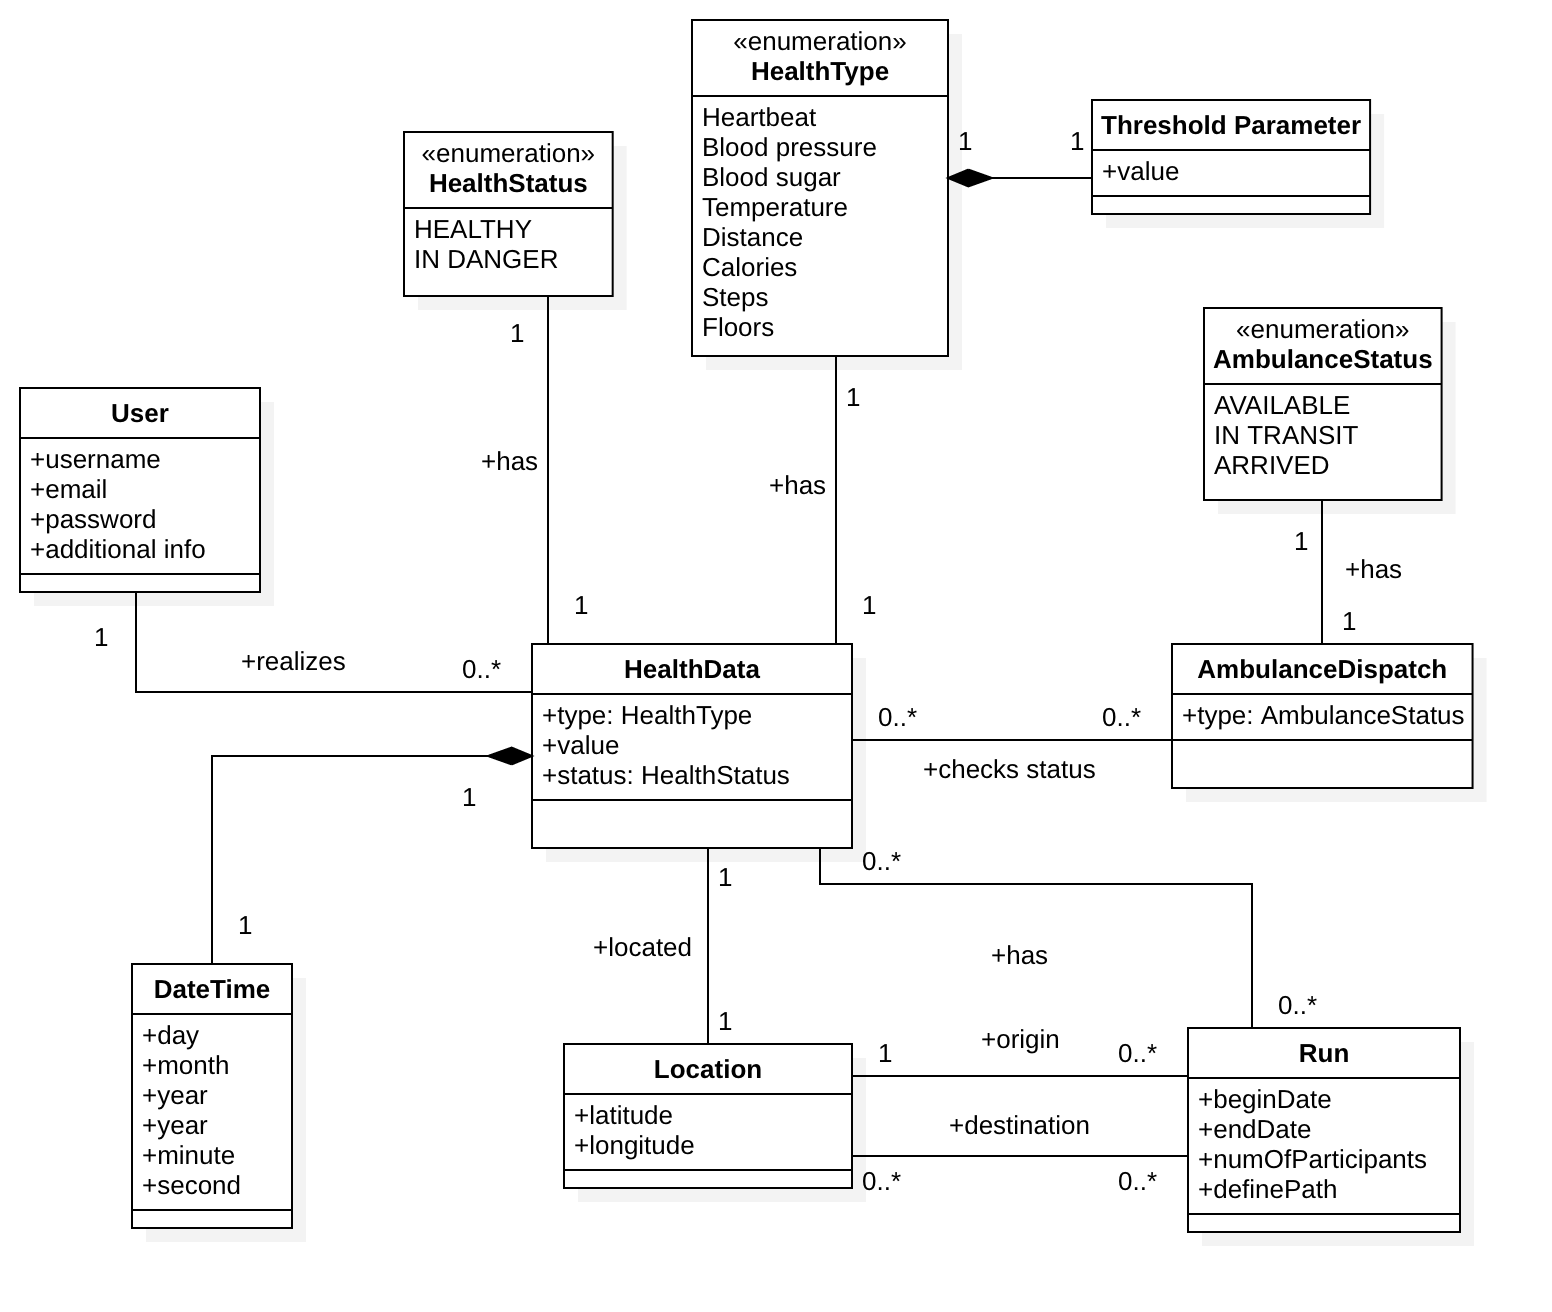
\includegraphics[scale=0.33]{classDiagram.png}
\label{fig:ClassDiagram}
\caption{Class Diagram of the domain.}
\end{figure}
\newpage

\begin{figure}[H]
\centering
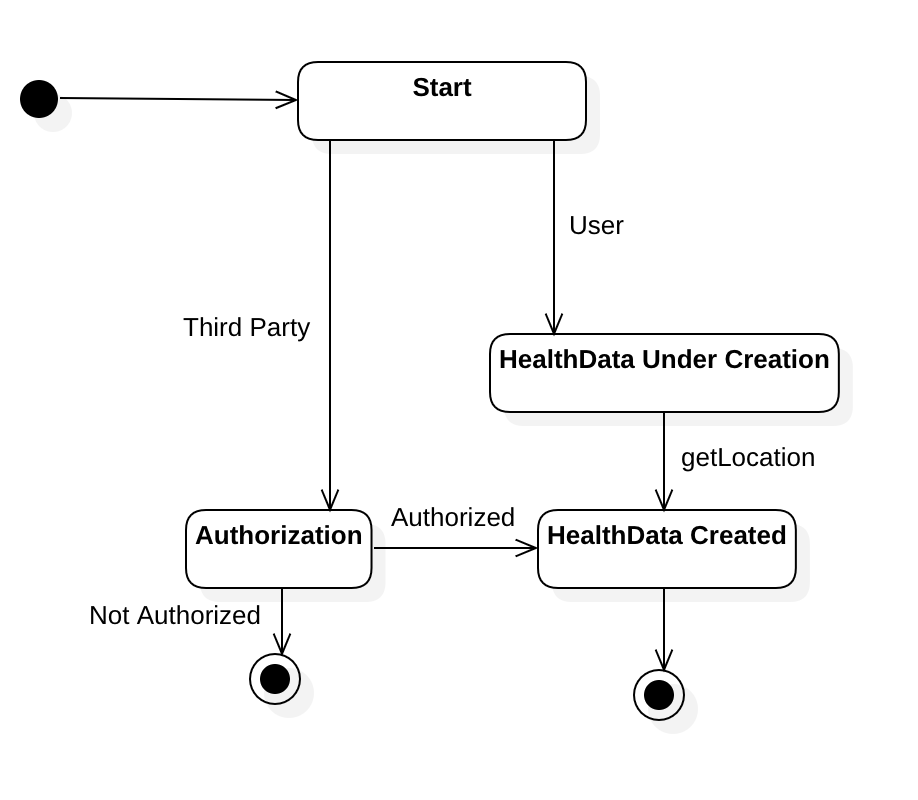
\includegraphics[scale=0.3]{Activity_D4H.png}
\label{fig:Activity_D4H}
\caption{Statechart of the Data4Help service.}
\end{figure}

\begin{figure}[H]
\centering
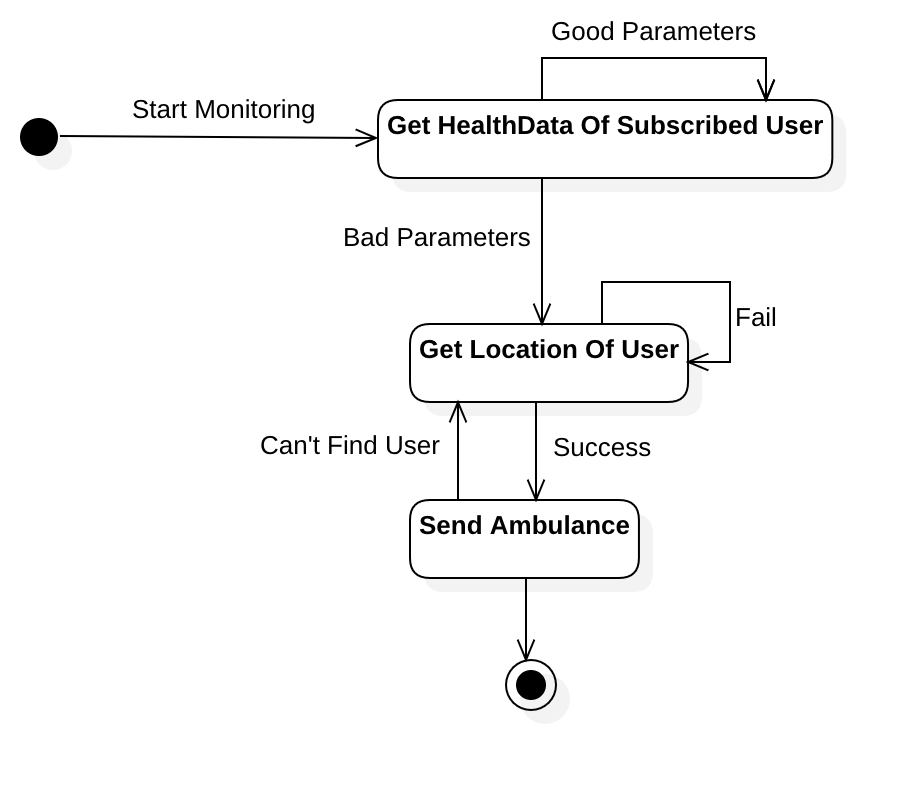
\includegraphics[scale=0.3]{Activity_SOS.png}
\label{fig:Activity_SOS}
\caption{Statechart of the AutomatedSOS service.}
\end{figure}

\begin{figure}[H]
\centering
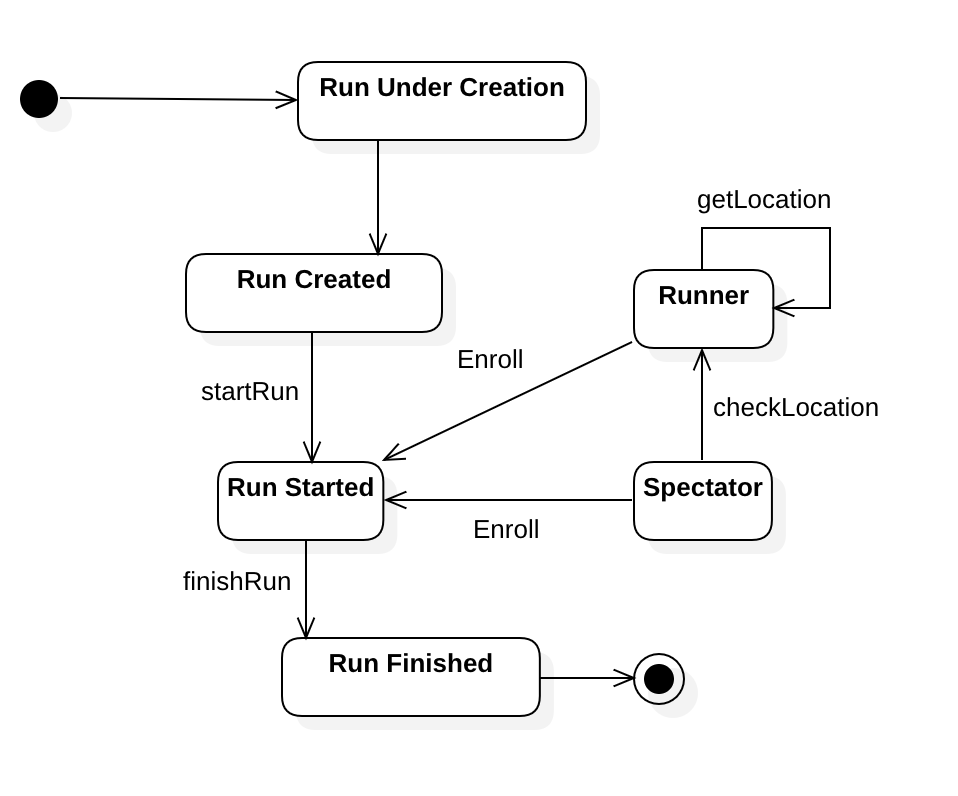
\includegraphics[scale=0.3]{Activity_T4R.png}
\label{fig:Activity_T4R}
\caption{Statechart of the Track4Run service.}
\end{figure}

\begin{figure}[H]
\centering
\includegraphics[scale=0.3]{commonstatediagram.png}
\label{fig:Activity_T4R}
\caption{Common state diagram.}
\end{figure}
\newpage
\subsection{Product Functions}
Considering all of the presented goals of the TrackMe system, the majority of functions of the system can be divided into 3 groups. In the following section, they are listed and more precisely specified, with respect to the already mentioned goals of the system.
\subsubsection{Data4Help}
The application gives you 2 types to login. The first way is the one to login as a user. The user can check his own location, track his motion path and time, and see health indicators. The second way is the one to login as a third party. A third party could check the location and health data of users by giving in an social security number (or something similar) of an individual. All these features combined form the Data4Help service.
\subsubsection{AutomatedSOS} This service also monitors the health parameters of subscribed individuals. When specific parameters are below a certain threshold it alarms an ambulance and the service passes them the location of the individual in danger. The service guarantees a reaction time less than 5 seconds from the time the parameters are below the threshold.
\subsubsection{Track4Run}
This service makes it possible for inidividuals to organize a certain path for a run comptetion. Individuals have also the possibility to join the run or track the location of all runners during the run. For monitoring the athletes who are participating in the run, the service exploits the features offered by Data4Help. 

\subsection{User Characteristics}
The system aims at satisfying the needs of two different types of users. The first type is the individual, the individual is the one who wants their health and location to be tracked and monitored. A lot of individuals will have several devices that track health data about them, this can be a smartphone, a smartwatch, etc. Therefore the purpose why individuals are using TrackMe, is that they need an application to improve the way their health data is being organized. They want to have one application where the data from all their devices is being displayed. The second type is the third party. A third party can be an organization like a hospital, a sporting company, etc. Their main purpose is that they need data to work with inside their organization. We assume that the individuals are people who are in possession of at least a smartphone or smartwatch. Therefore we set the age of our individuals, who will use the application, between 10 and 80 years old.

\subsection{Assumptions, dependencies and constraints}
[D1] The username and email must be unique. \newline
[D2] The system will have access to the smartphone/smartwatch GPS functionality. \newline
[D3] The phone will always have a connection to the internet (WiFi or mobile data). \newline
[D4] Individuals are using a smartwatch and a smartphone to monitor the health status. They can have additional devices to monitor specific paramaters but this is not necessary.\newline
[D5] Individuals accept to share their data with the application's online database. \newline
[D6] The external services used by the system are assumed to be always available and reachable. \newline
[D7] The threshold of the health status parameters are fixed unless an individual/third party changes them. \newline
[D8] Data (health or location) maps only to one specific inidividual. \newline
[D9] The location of individuals is always known by the system. \newline
[D10] General info (length, weight, gender, date of birth, fiscal code) is given by the individual upon registration. \newline


\subsubsection{Hardware limitations}
\begin{itemize}
    \item Mobile application
    \begin{itemize}
        \item iOS or Android smartphone
        \item 2G/3G/4G connection
        \item GPS
    \end{itemize}
    \item Devices
    \begin{itemize}
        \item Smartphone
        \item Smartwatch
        \item Blood sugar control device
        \item Thermometer
        
    \end{itemize}
\end{itemize}

\section{Specific Requirements}

\subsection{External Interface Requirements}

\subsubsection{User Interfaces}


The following Mockups represent a basic idea of how the systems user interface will look like on the first release (mobile application):
\begin{itemize}
    \item Figure 1 and 2 show the login screen and registration screen for an individual and a third party.
    \item Figure 3 shows the different windows you have in the home screen. The first screen is today's activities, activities like for example walked and running distance are showed for a specific day. The second screen is health data where we can find detailed information about an individual such as hearthbeat, blood pressure, etc. In figure 4 (left) we find the third screen, the one who makes it possible to make/enroll/spectacte a run. These screens are only available for indivduals. The right screen in figure 4 is ment to be for third parties. They can enter a fiscal code of an individual they want to track and enter a data request as well. 
    \item The AutomatedSOS doesn't need an extra user interface. In the background the system monitors  the health status of an individual through Data4Help and when the individual is in danger, a parameter is lower than the threshold of that certain parameter, a popup occurs on the home screen saying the system noticed an unusual event and sends an ambulance to the specific individual.
\end{itemize}

\newpage
\begin{figure}[t!]
\centering
    \begin{subfigure}{.4\textwidth}
        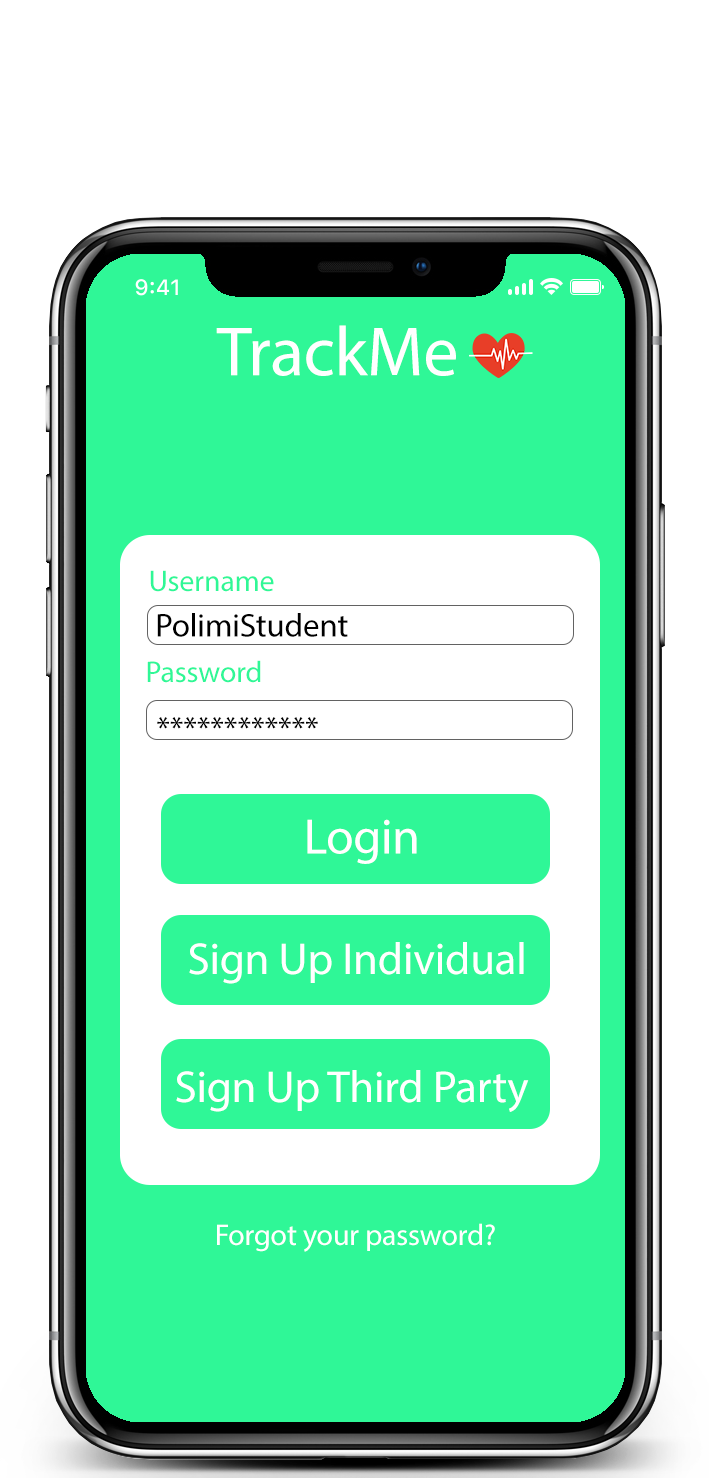
\includegraphics[scale=0.2]{LoginScreen.png}
        \label{fig:loginScreen}
    \end{subfigure}%
    \begin{subfigure}{.4\textwidth}
        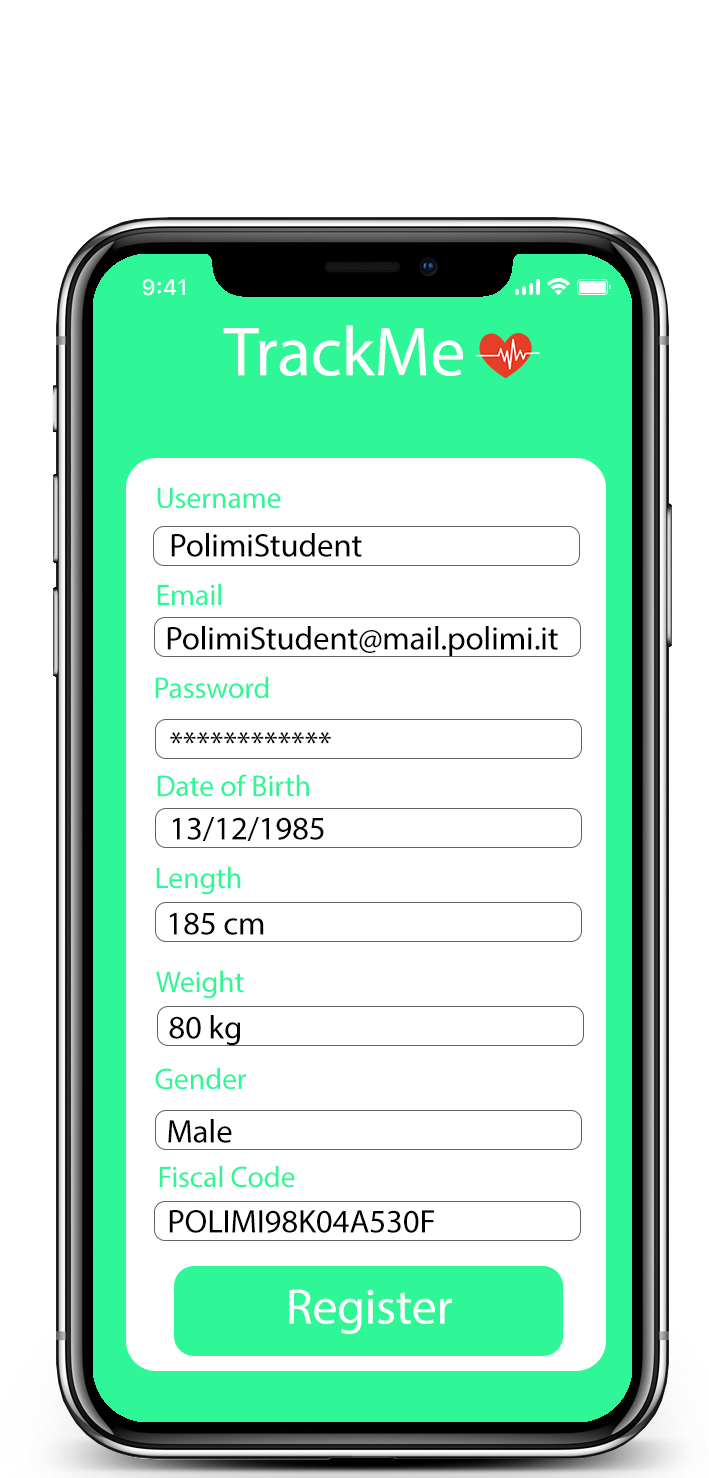
\includegraphics[scale=0.2]{RegisterScreen-Individual.png}
        \label{fig:RegisterScreen-Individual}
    \end{subfigure}
    \caption{Login Screen (left) and  Register Screen for an individual (right)}
\end{figure}

\begin{figure}[H]
\centering
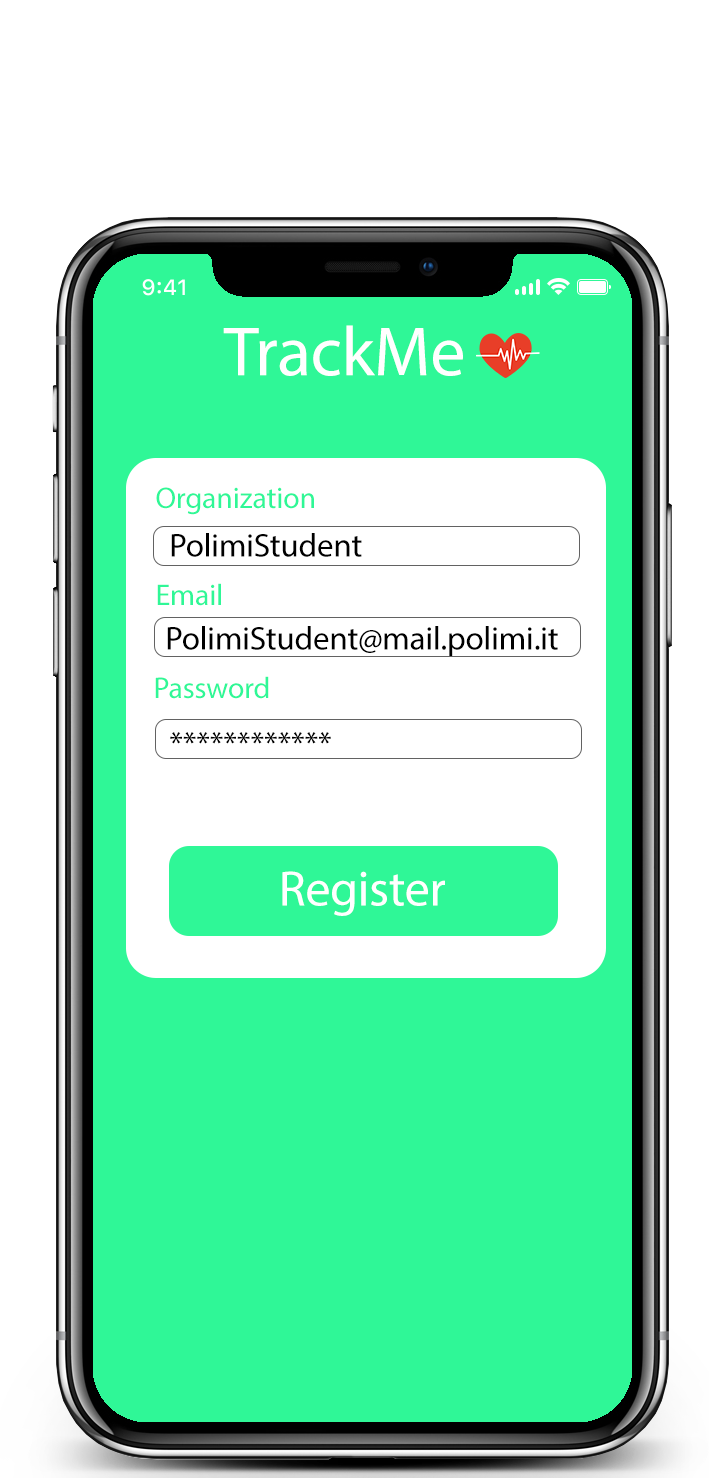
\includegraphics[scale=0.2]{RegisterScreen-ThirdParty.png}
\label{fig:RegisterScreen-ThirdParty}
\caption{Register Screen for a Third Party.}
\end{figure}

\begin{figure}[t!]
\centering
    \begin{subfigure}{.4\textwidth}
        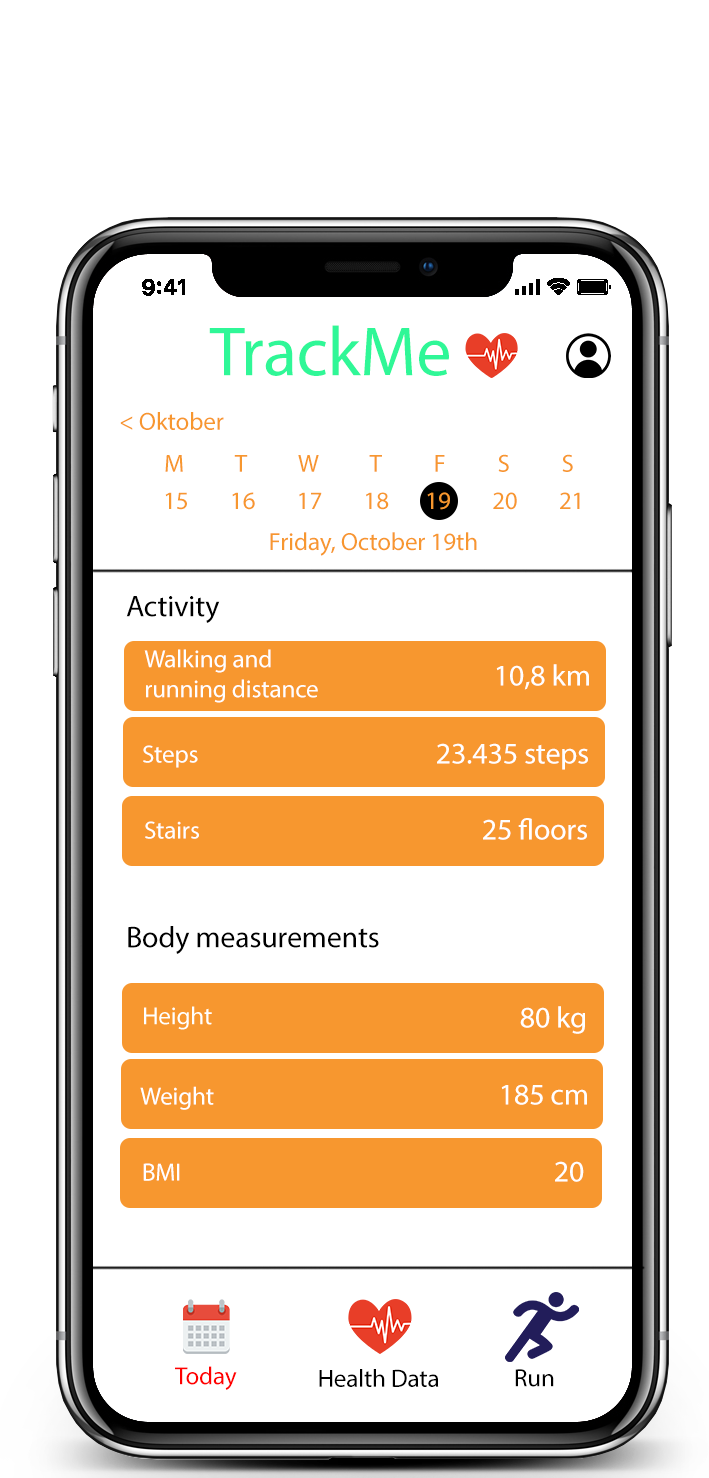
\includegraphics[scale=0.2]{HomeScreen1.png}
        \label{fig:HomeScreen1}
    \end{subfigure}%
    \begin{subfigure}{.4\textwidth}
        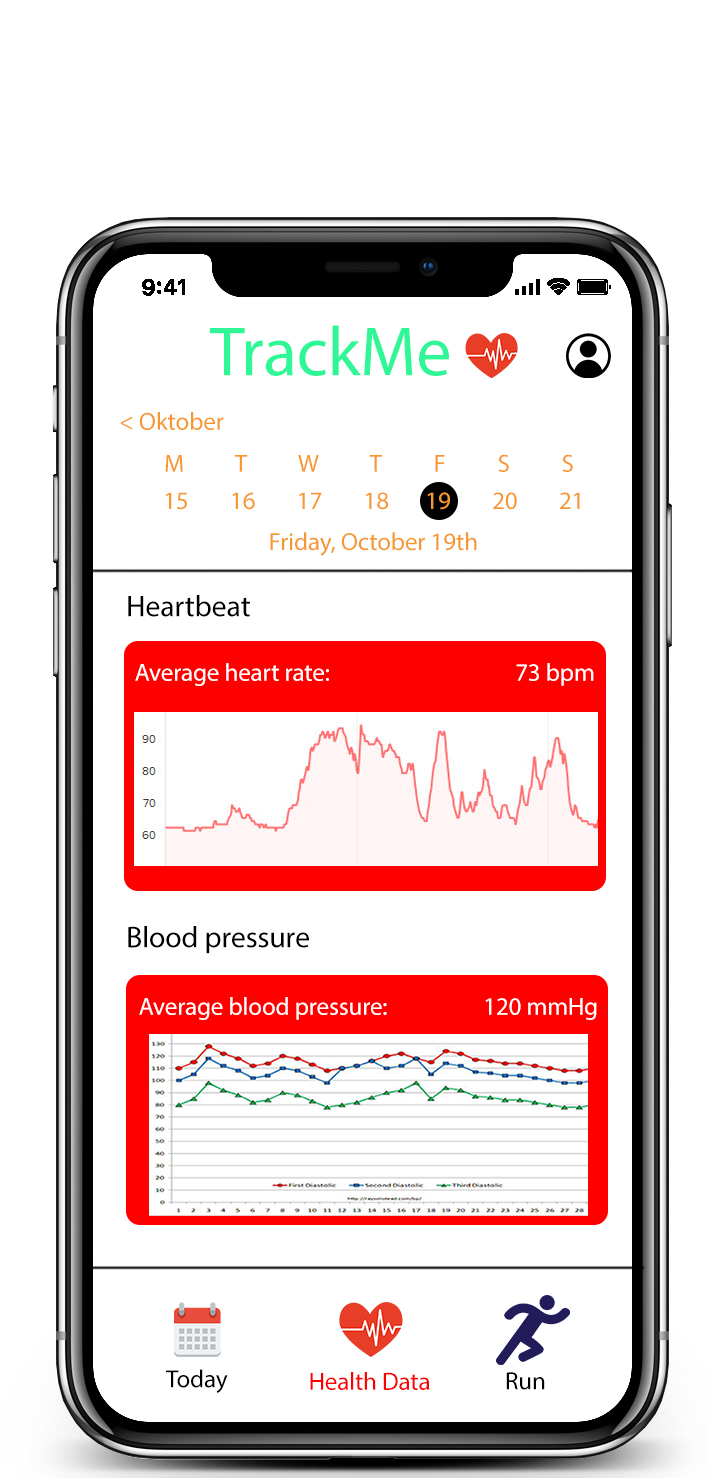
\includegraphics[scale=0.2]{HomeScreen2.png}
        \label{fig:HomeScreen2}
    \end{subfigure}
    \caption{Home Screen: Today's activities (left) and Health Data (right)}
\end{figure}

\begin{figure}[H]
\centering
    \begin{subfigure}{.4\textwidth}
        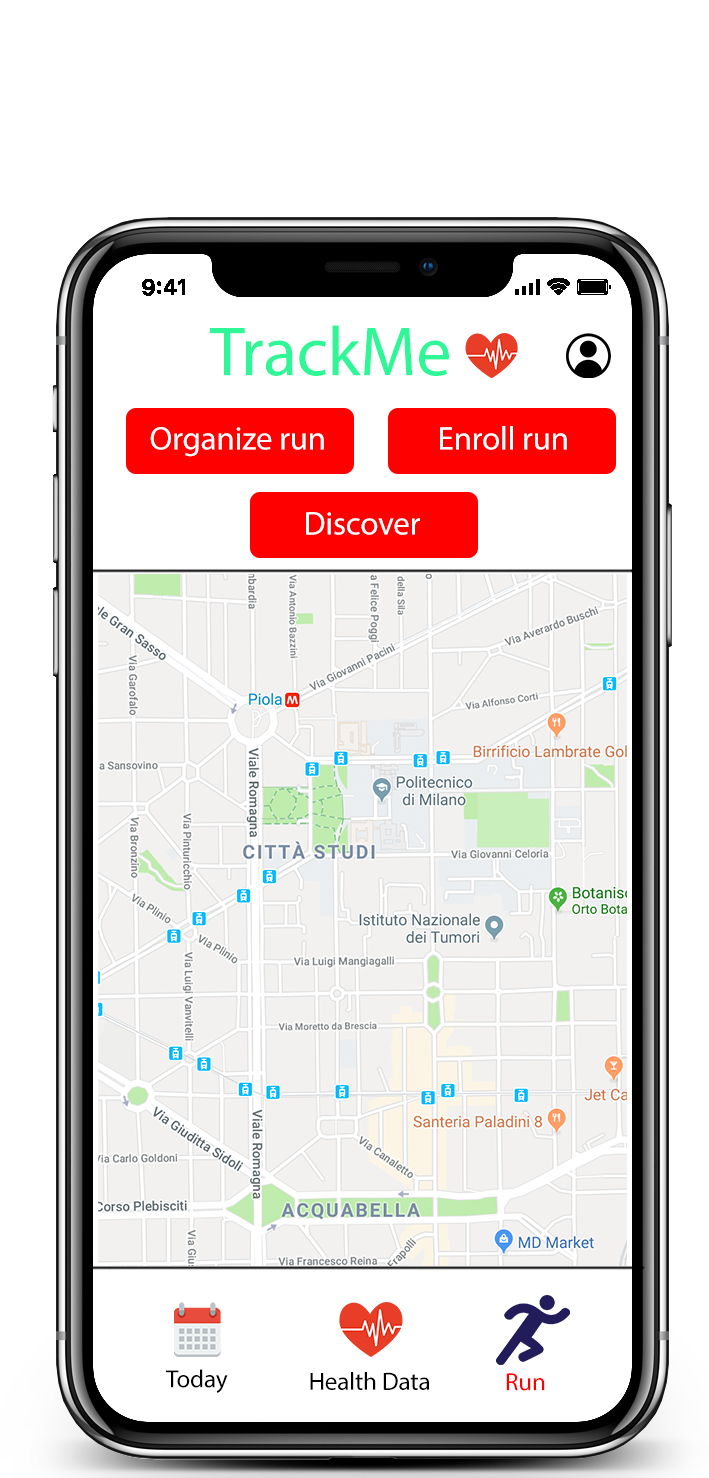
\includegraphics[scale=0.2]{HomeScreen3.png}
        \label{fig:HomeScreen1}
    \end{subfigure}%
    \begin{subfigure}{.4\textwidth}
        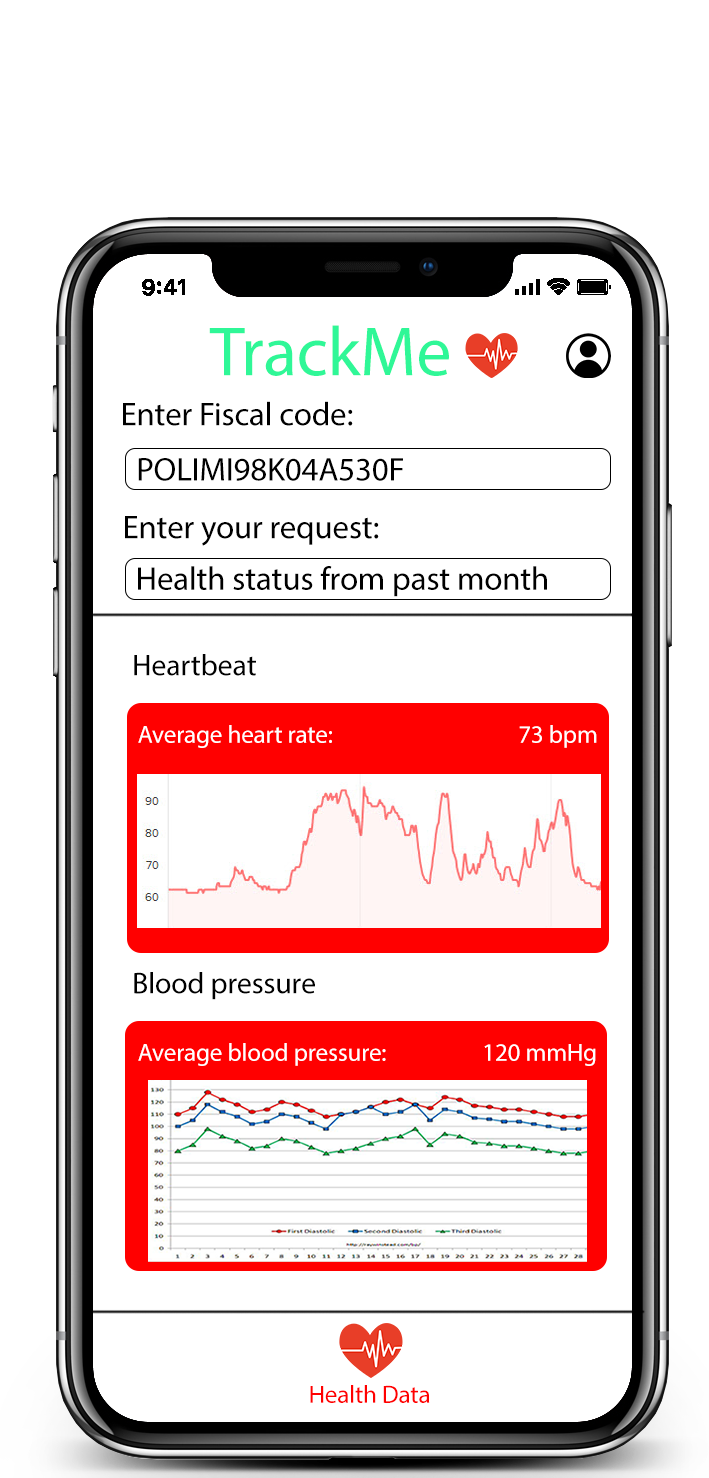
\includegraphics[scale=0.2]{HomeScreen4.png}
        \label{fig:HomeScreen2}
    \end{subfigure}
    \caption{Home Screen for individual (left) and for a third party (right)}
\end{figure}


\subsubsection{Hardware Interfaces}
In the first release, no Hardware Interfaces will be necessary since the system doesn’t need to interact physically with other systems.
\subsubsection{Software Interfaces}
Given the wide range of features the system offers, it will need to have several software interfaces. There has to be a way of storing all the user-related data (mainly login, general info, location and health data). In that sense, the system will use a \textbf{MySQL API} to connect with our MySQL database server, where all the application data will be stored. The system will also need different kinds of information about the individuals location, in order to combine health data with a location. To support this functionality, the system will use \textbf{Google Maps Geolocation API} and \textbf{Google Maps API}. The first one will provide information about the individual exact location and the second one will provide the real-time information about maps. The last will allow individuals to define a path for a run and for others to see the route for the run. To have access to the ambulance dispatch system and send them a request for an ambulance if an individual is in danger, our system will have an interface with \textbf{Ambulanza Milano}. At last, all the health data will come from several different devices and possibly from other brands as well. To gather all this health data we need to use serveral API's. Since a lot of devices (smartwatch, blood pressure device, ...) are seamlessly working with iOS and Android we need to communicate with iOS and Android API's. Considering a lot of third party applications who offer a specific health tracking application, like measuring the blood control for a diabetic person, work with \textbf{HealthKit} and \textbf{Google Fit}, we will mainly use these two for keeping track of the health status of the individuals. 

\subsubsection{Communication Interfaces}
Communication interfaces ensure the communication between the system and the other software interfaces (third party service providers). The communication between the system and those service providers is crucial because the system depends on those services to perform its functions. Given this, the systems communication interface must be either WiFi or Mobile Data (2G, 3G or 4G), and the service providers communication interface can be of any type, as long as it ensures that they are connected to the internet. The protocol used shall be HTTPS, in order to keep the communications secure.

\subsection{Functional Requirements}
\subsubsection{Data4Help}
[G1] Allow a visitor to become a registered individual or third party after providing email, username/organization, password, general info (if case of an individual). \newline
\begin{itemize}
    \item{[R1]} The system shall allow the visitor to begin the registration process when he accesses the system.
    \item{[R2]} The system shall ask the visitor for the required information and credentials during the registration process.
    \item{[R3]} The system shall register the visitor as a individual or third party when the registration process ends, if all the data inserted by the visitor is valid.
    \item{[R4]} The system shall not allow a visitor to access more than the registration functionality.
\end{itemize}
[G2] Allow a user to monitor it's health status.\newline 
\begin{itemize}
    \item {[R5]} The system can receive data from external devices. 
    \item {[R6]} The system can store received data. 
    \item {[R7]} The system allows users to access its own data whenever it wants.
\end{itemize}
[G3] Allow third parties to request data from a specific individual after authorization.\newline 
\begin{itemize}
    \item {[R8]} The system shall allow registered users to ask individaul permission to access data.
    \item {[R9]} The system shall allow individual to accept or refuse the request. 
    \item {[R10]} A third party can access data only from individuals that accept their request.
    \item {[R11]} When a third party gets the authorization to access data from an individual it can always access those data. 
\end{itemize}
[G4] Allow third parties to subscribe to new data and receive them as soon as they are produced.\newline
\newpage
[G5] Allow third parties to access anonymized data of a group of individuals.\newline 
\begin{itemize}
    \item {[R12]} A third party can ask the system to access data of a group of individuals, by entering their fiscal code. 
    \item {[R13]} The system allows a third party to access data of a group only if the number of individuals is greater than 1000. 
\end{itemize}
[G6] Allow individuals to choose what data is being send to the application's DB.\newline 
\begin{itemize}
    \item {[R14]} An individual can choose what data he wants to send to the application.
    \item {[R15]} At any time an individual can change the data they would like to send to the application.
    \item {[R16]} When an individual decides to stop sending certain data to application, a third party cannot access it anymore.  
\end{itemize}
\subsubsection{AutomatedSOS}
The folowing goals and requirements are specific to the AutomatedSOS service, the goals and requirements of the Data4Help service also hold here.
\vspace{2mm}
\newline
[G7] Allow third parties to acquire data from Data4Help.\newline 
\begin{itemize} 
    \item {[R17]} AutomatedSOS uses the same DB as Data4Help.
\end{itemize}
[G8] Allow individuals to define a certain threshold for a certain parameter.\newline 
\begin{itemize}
    \item {[R18]} At the very beginnnig thresholds are default fixed.
    \item {[R19]} An Individual can change his thresholds at any time depending on its health status.  
\end{itemize}
[G9] Call an ambulance when parameters drop below a certain threshold.\newline
\begin{itemize}
    \item {[R20]} The system monitors health status of an individual every 30 seconds. 
    \item {[R21]} The system is connected with an ambulance dispatch.
    \item {[R22]} When health parameters of an individual drops below the threshold the system calls an ambulance.
\end{itemize}
\subsubsection{Track4Run}
The folowing goals and requirements are specific to the Track4Run service, the goals and requirements of the Data4Help service also hold here.
\vspace{2mm}
\newline
[G10] Allow an individual/third party to organize a track for a run.\newline
\begin{itemize}
    \item {[R23]} Allow an individual/third party to define a track through a map. 
    \item {[R24]} The system checks if the track is feasible.
    \item {[R25]} The system calculates the length of the track. 
\end{itemize}
[G11] Allow an individual/third party to enroll for a run.\newline 
\begin{itemize}
    \item {[R26]} The system shows all ongoing runs that are organized in a certain period and place. 
    \item {[R27]} Allow individuals/third parties to decide to enroll for a run as runners or spectators.
\end{itemize}
[G12] Allow an individual/third party to see the live position of all runners during the run.\newline 
\begin{itemize}
    \item {[R28]}The system shows in real-time the position on the map of all participating runners.
\end{itemize}
\subsubsection{Use Case Diagrams}

\begin{figure}[H]
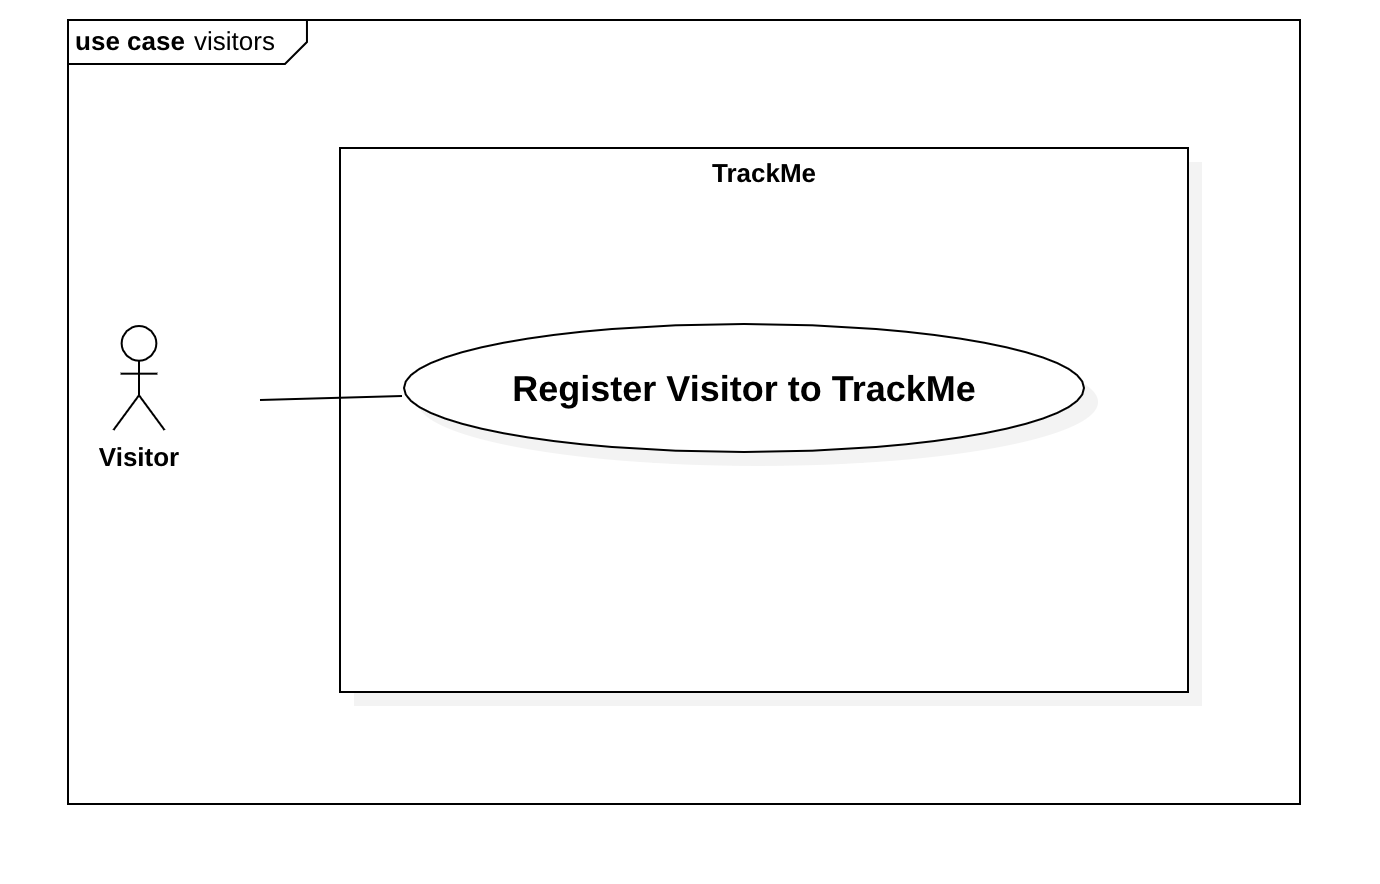
\includegraphics[scale=0.25]{VisitorUseCase.png}
\centering
\label{fig:VisitorUseCase}
\caption{Visitor Use Case.}
\end{figure}

\begin{figure}[H]
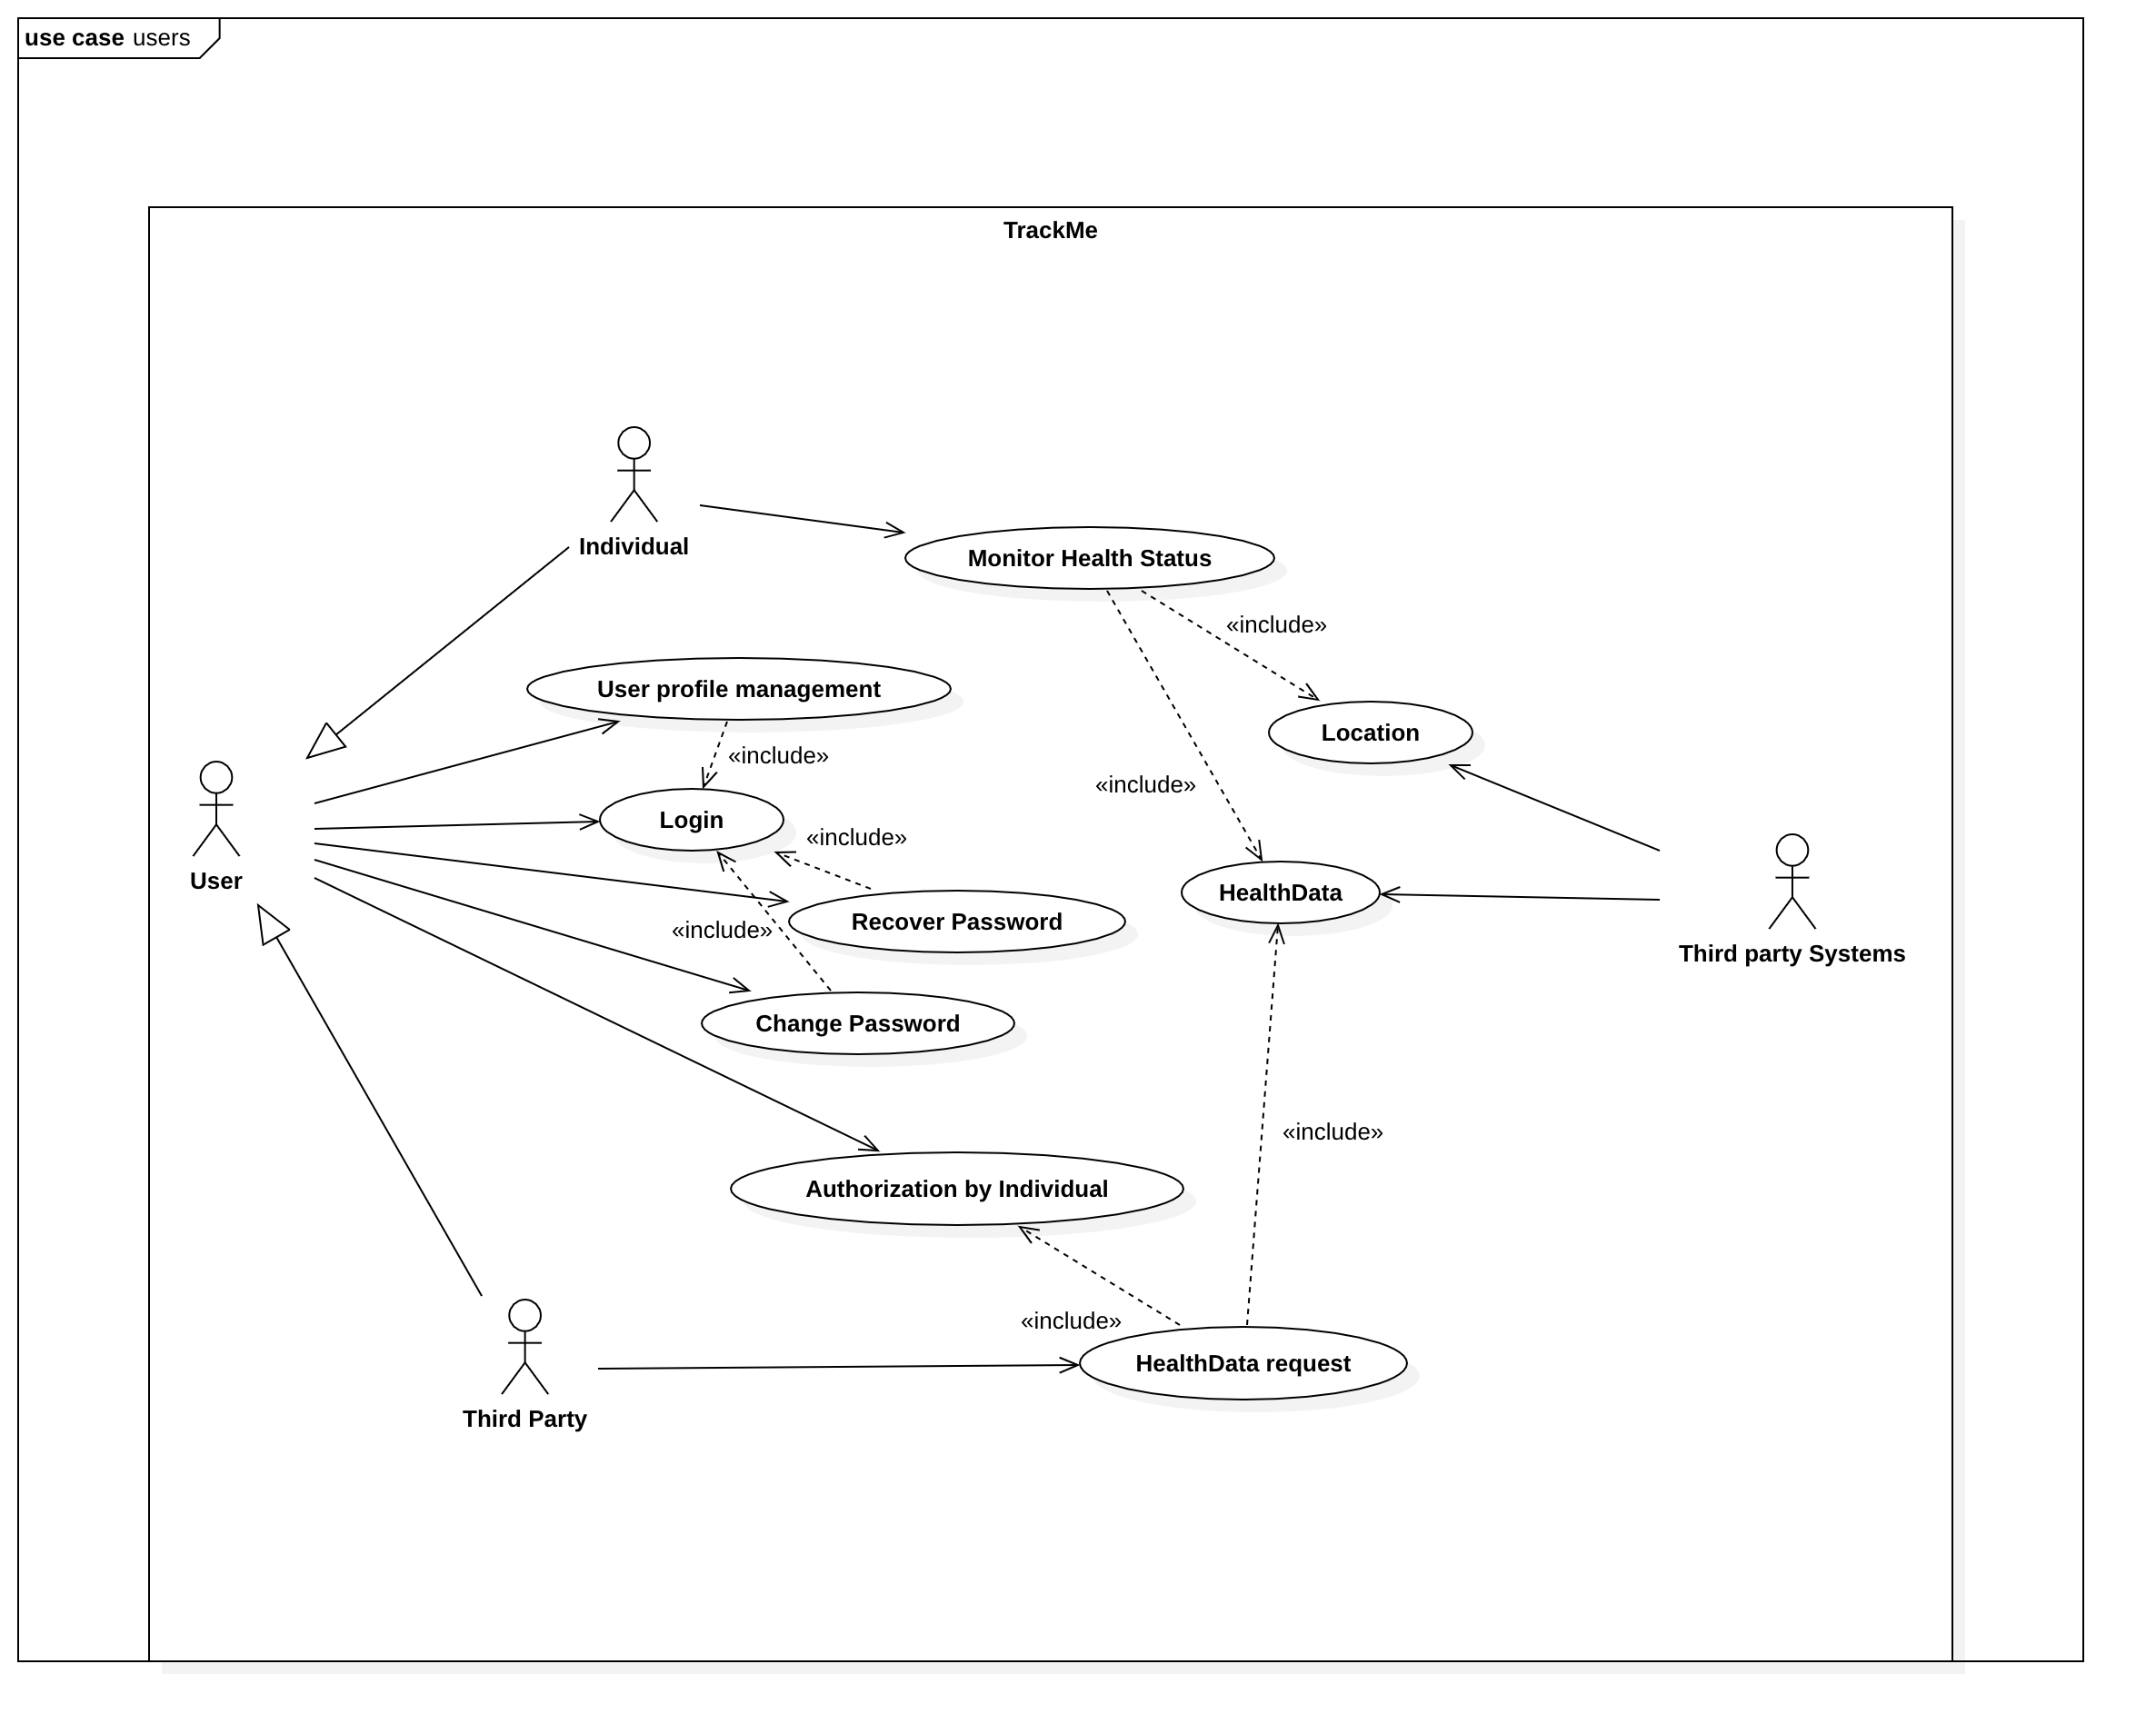
\includegraphics[scale=0.2]{UseCase-Data4Help.png}
\centering
\label{fig:UseCase-Data4Help}
\caption{User use case for the Data4Help service.}
\end{figure}

\begin{figure}[H]
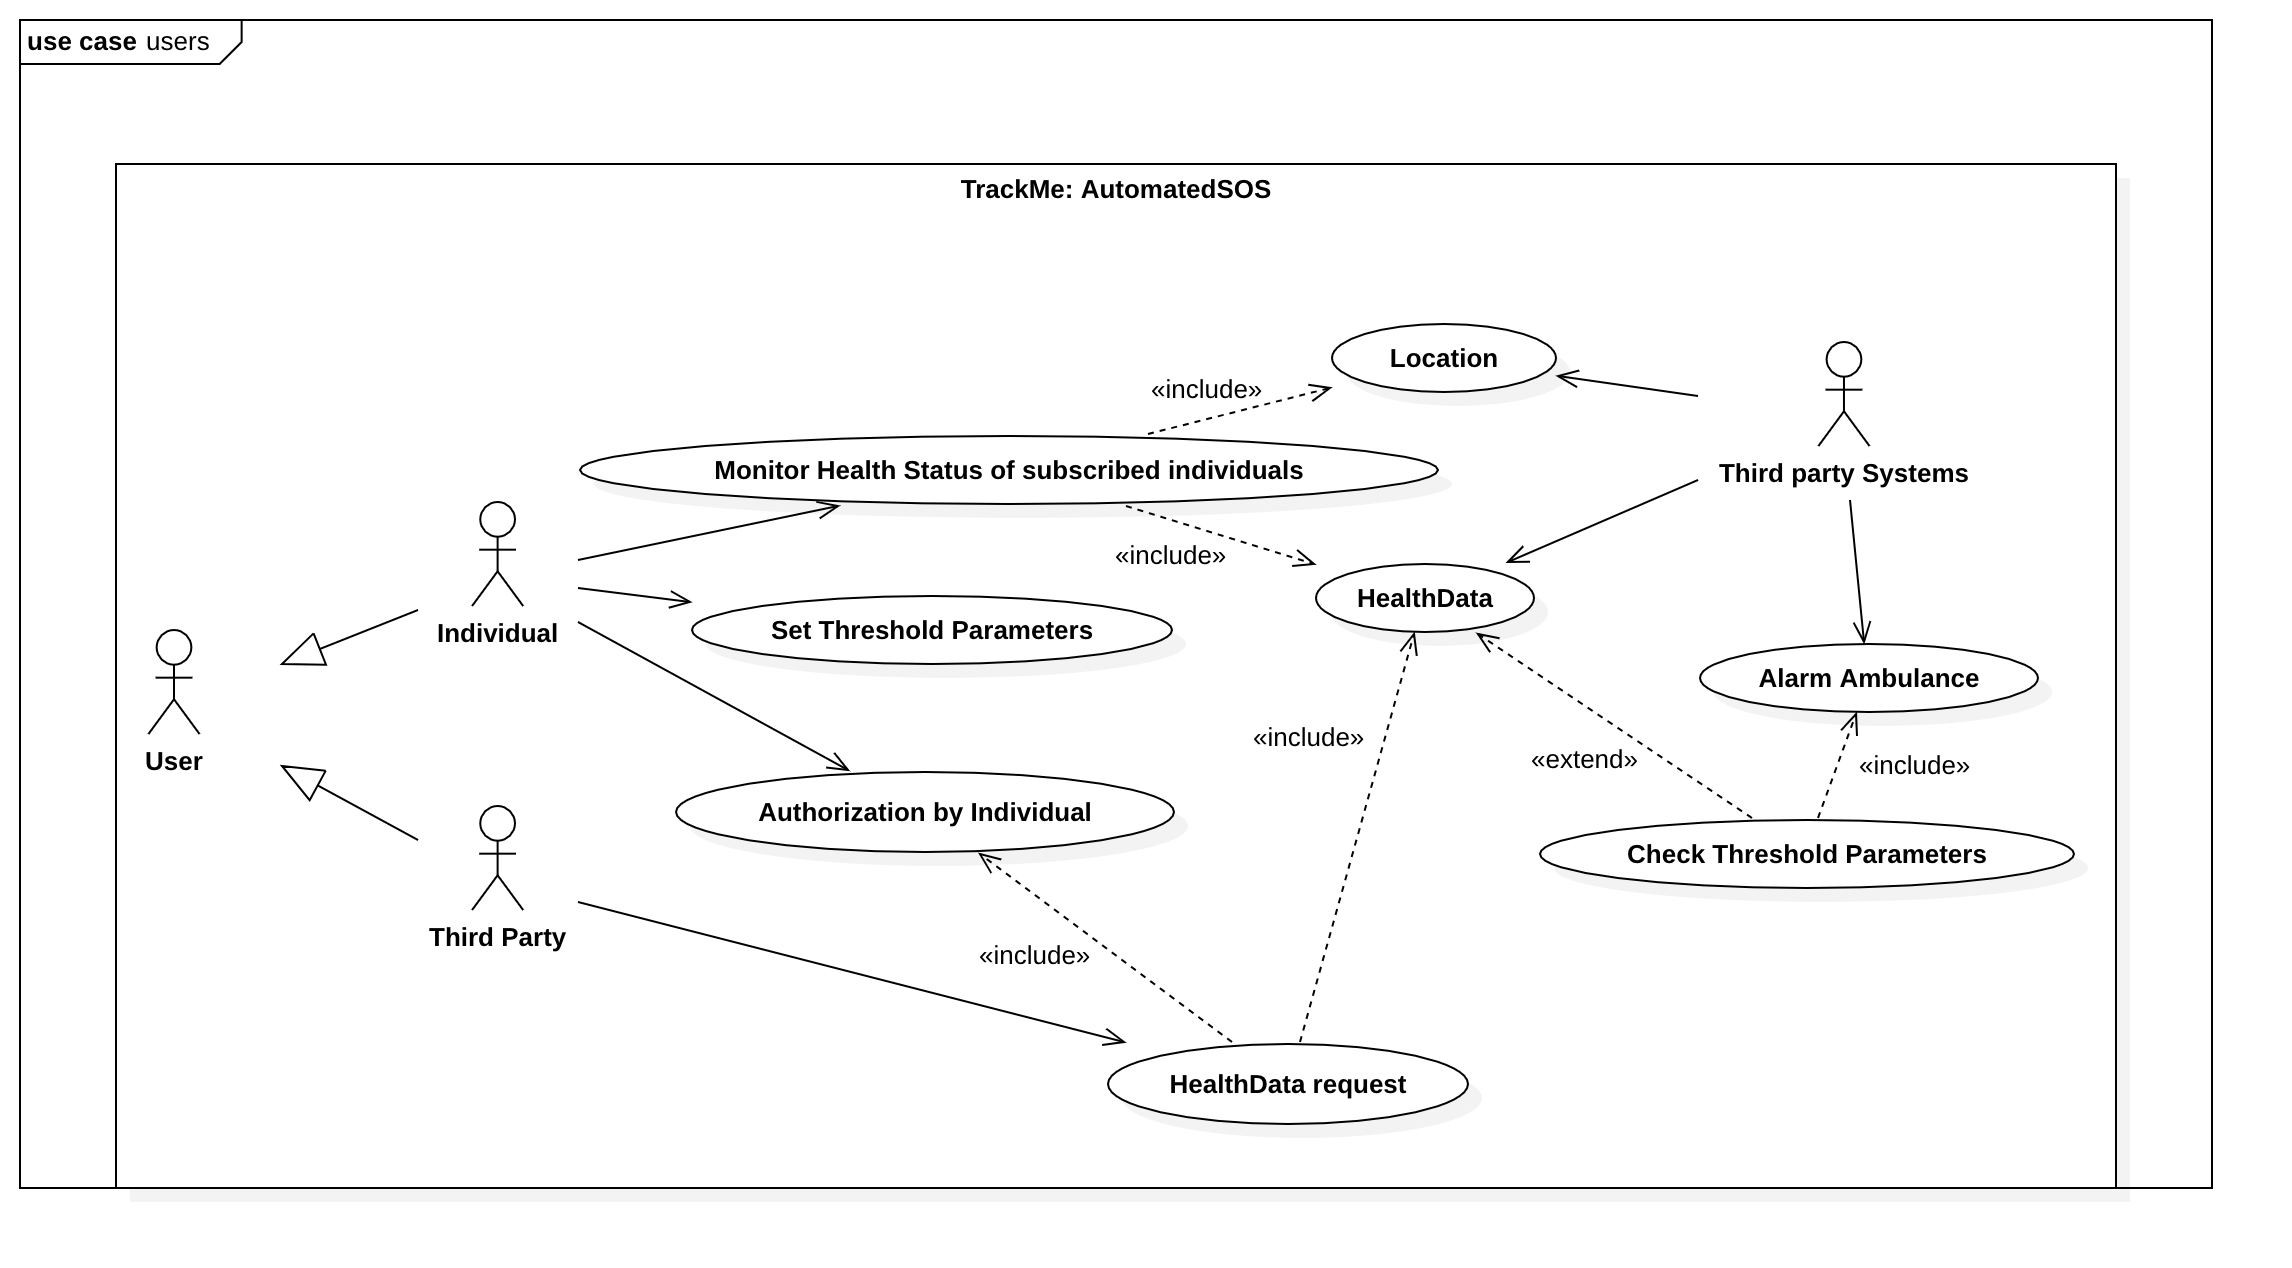
\includegraphics[scale=0.2]{UseCase-AutomatedSOS.png}
\centering
\label{fig:UseCase-AutomatedSOS}
\caption{User use case for the AutomatedSOS service.}
\end{figure}

\begin{figure}[H]
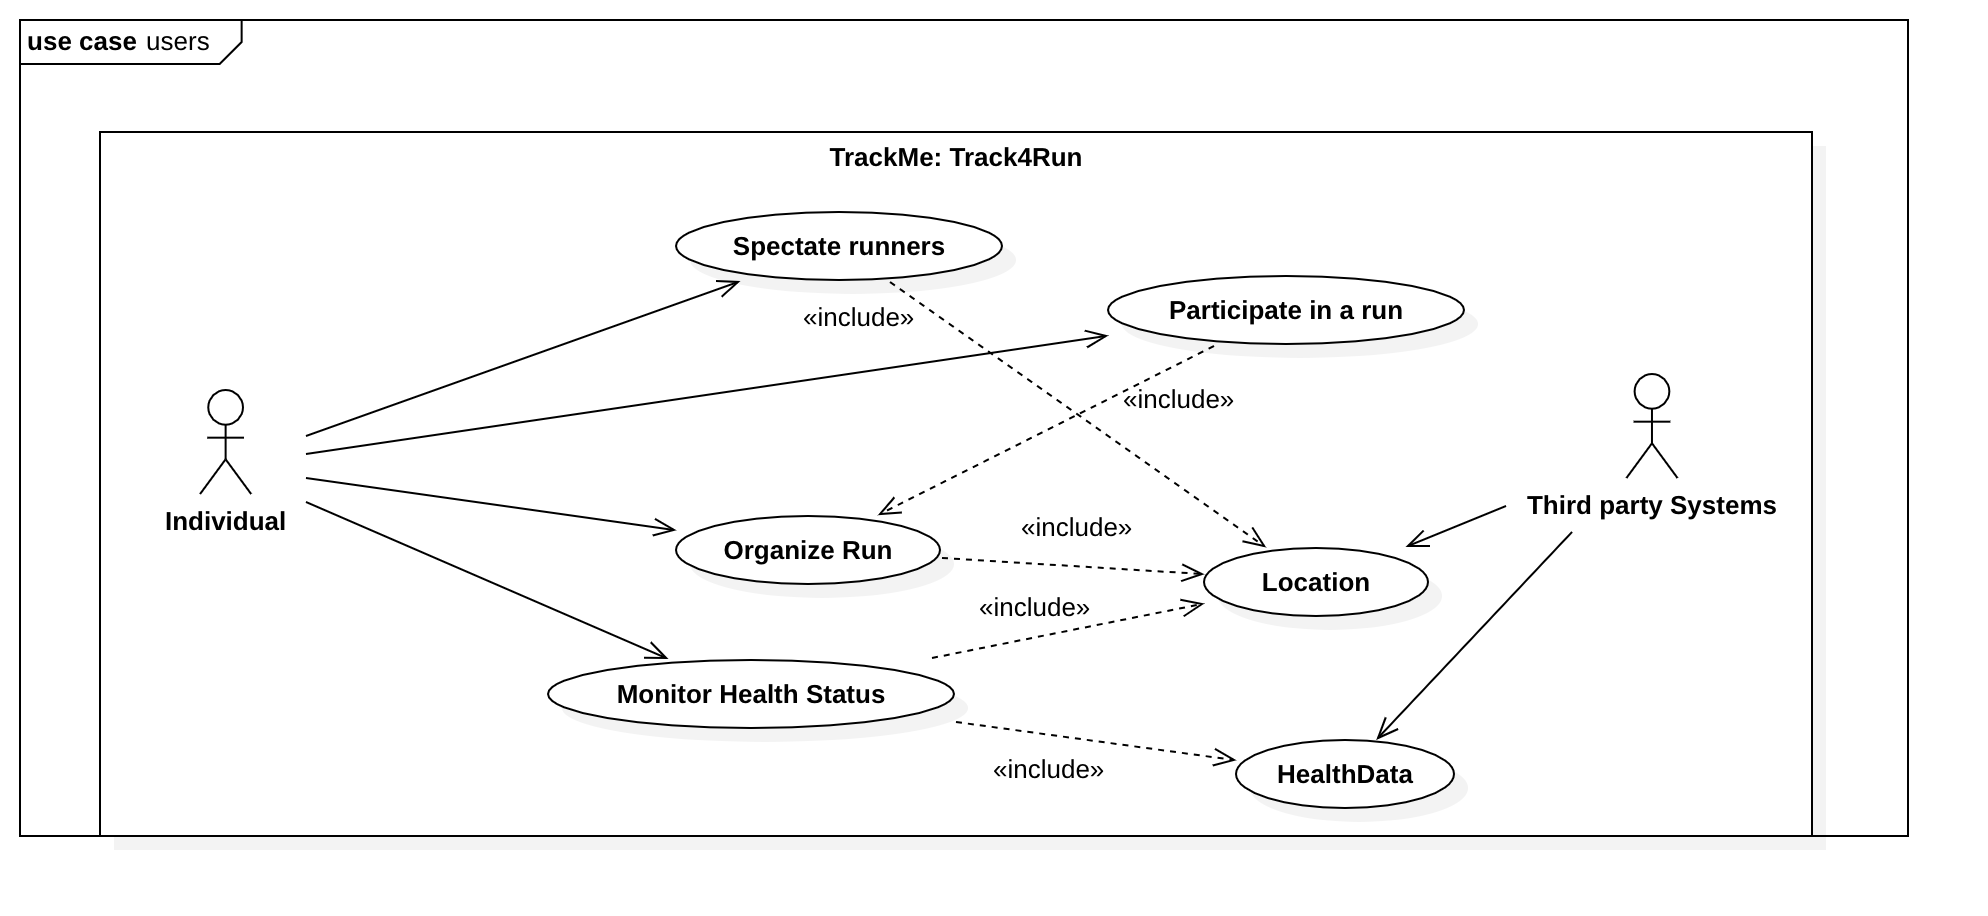
\includegraphics[scale=0.25]{UseCase-Track4Run.png}
\centering
\label{fig:UseCase-Track4Run}
\caption{User use case for the Track4Run service.}
\end{figure}

\subsubsection{Use Case Description}
\paragraph{Visitor Registration}

\begin{center}
    \begin{tabular} { |p{0.25\textwidth}|p{0.8\textwidth}| }
        \hline
        \textbf{Actors} & Visitor \\ 
        \hline
        \textbf{Goals} & {[G1]} \\ 
        \hline  
        \textbf{Preconditions} & There are no preconditions. \\ 
        \hline
        \textbf{Events Flow} & \begin{enumerate}[topsep=0pt]
                            \setlength{\itemsep}{0.5pt}
                            \item The visitor opens the TrackMe application.
                            \item The visitor clicks on the "Sign up Individual" button in case of an inidividual and on the "Sign up Third Party" in case of a third party button to start the registration process.
                            \item The system provides the Visitor a form with the required data fields which need to be filled in order for him to be registered as a individual/Third party.
                            \item The visitor fills the fields with his data. 
                            \item The visitor clicks on the "Register Button", submitting the data to the system.
                            \item The system verifies if all the data are valid.
                            \item The system saves the data in an online DB.
                            \item The system notifies the Visitor that his registration as a individual/Third party has been completed with success, and redirects him to the right Home Screen (depends on which type of user is registering).
                            \end{enumerate} \\
        \hline
        \textbf{Postconditions} & The visitor ends the registration process successfully and from now on is a user of the system, being able to access all of its functionality. \\
        \hline
        \textbf{Exceptions} & \begin{enumerate}[topsep=0pt]
                            \setlength{\itemsep}{0.5pt}
                            \item The visitor is already an existing individual or third party. 
                            \item The visitor doesn't fill all the mandatory fields or fills them with invalid data.
                            \item The visitor chooses a username/organization or email which is already associated with another individual or third party.
                            \end{enumerate} 
                            All exceptions are handled notifying the visitor about the issue and going back to the applications initial screen.\\ 
        \hline
    \end{tabular}
\end{center}
\newpage
\paragraph{User login}
\begin{center}
    \begin{tabular} { |p{0.25\textwidth}|p{0.8\textwidth}| }
         \hline
         \textbf{Actors} & User \\ 
         \hline
         \textbf{Goals} & All goals except [G1] \\ 
         \hline  
         \textbf{Preconditions} & There are no preconditions. \\ 
         \hline
         \textbf{Events Flow} & \begin{enumerate}[topsep=0pt]
             \setlength{\itemsep}{0.5pt}
             \item The user opens the TrackMe application.
             \item The user inserts his username and password on the respective fields.
             \item The user clicks on the ”Log In” button.
             \item The system validates the user credentials.
             \item The system redirects the user to the Home Screen.
             \end{enumerate} \\ 
        \hline
        \textbf{Postconditions} & The user is successfully logged in to the system and redi- rected to the Home Screen. \\
        \hline 
        \textbf{Exceptions} & \begin{enumerate}[topsep=0pt] 
              \setlength{\itemsep}{0.5pt}
              \item The user inserts an invalid username.
              \end{enumerate}
              All exceptions are handled notifying the User about the issue and going back to event 2 of the Event Flow described above.\\ 
        \hline
    \end{tabular}
\end{center}



\newpage
\paragraph{Third Party request to access data}
\begin{center}
    \begin{tabular} { |p{0.25\textwidth}|p{0.8\textwidth}| }
         \hline
         \textbf{Actors} & Third Party \\ 
         \hline
         \textbf{Goals} & {[G3]} \\ 
         \hline  
         \textbf{Preconditions} & The third party has to be already logged in. \\ 
         \hline
         \textbf{Events Flow} & \begin{enumerate}[topsep=0pt]
             \setlength{\itemsep}{0.5pt}
             \item The third party opens TrackMe application.
             \item The third party clicks on Enter Fiscal code button.
             \item The third party insert fiscal code of Individual that wants to monitors.
             \item The third party clicks on Enter your Request button. 
             \item The third party specifies its request.
             \item The system sends request to Individual specified by fiscal code.
             \item After authorization, the system downloads data from its online database and displays them on the third party screen.
             \end{enumerate} \\ 
        \hline
        \textbf{Postconditions} & The third party can see all the data that he requires from the Individual that has specyfied before. \\
        \hline 
        \textbf{Exceptions} & \begin{enumerate}[topsep=0pt] 
              \setlength{\itemsep}{0.5pt}
              \item The fiscal code is wrong and does not exixt any Individual associated with that fiscal code. 
              \item The Individual does not accept the request of third party. 
              \item The request is different from the ones that the system can manage. 
              \end{enumerate}
               All exceptions are handled notifying the visitor about the issue and going back to the applications initial screen.\\ 
        \hline
    \end{tabular}
\end{center}
  
  
\newpage              
\paragraph{ The system calls an ambulance} 
\begin{center}
    \begin{tabular} { |p{0.25\textwidth}|p{0.8\textwidth}| }
         \hline
         \textbf{Actors} & The system \\ 
         \hline
         \textbf{Goals} & {[G9]} \\ 
         \hline  
         \textbf{Preconditions} & The Individual must be subscribed, the location of the Individual must be available and the system must be able to call an ambulance. \\ 
         \hline
         \textbf{Events Flow} & \begin{enumerate}[topsep=0pt]
             \setlength{\itemsep}{0.5pt}
             \item The system accesses to the online DB.
             \item The system automatically checks health paramaters of the Individual 
             \item The system realizes that some health parameters are below a certain threshold. 
             \item The system checks the position of the Individual. 
             \item The system calls the ambulance dispatcher in order to have an ambulance. 
             \item The systems sends the health status and location of the Individual to the ambulance dispatcher. 
             \end{enumerate} \\ 
        \hline 
        \textbf{Postconditions} & The SSN is informed that there is a people in danger, knows its location and its health status. \\ 
        \hline
         \textbf{Exceptions} & \begin{enumerate}[topsep=0pt] 
              \setlength{\itemsep}{0.5pt}
              \item Position of Individual is not available. 
              \item Data from Individual are not considered to be reliable. 
              \end{enumerate}
            In order to manage the first exeption the system must to try again to relocate Individual while it is calling the ambulance dispatcher. In the second case it could do another check and then call the ambulance dispatcher. \\
             \hline
    \end{tabular}
\end{center}

\newpage
\paragraph{An Individual organizes a run} 
\begin{center}
    \begin{tabular} { |p{0.25\textwidth}|p{0.8\textwidth}| }
         \hline
         \textbf{Actors} & Individual \\ 
         \hline
         \textbf{Goals} & {[G10]} \\ 
         \hline  
         \textbf{Preconditions} & Individual must be subscribed to the system and the maps must be available \\ 
         \hline
         \textbf{Events Flow} & \begin{enumerate}[topsep=0pt]
             \setlength{\itemsep}{0.5pt}
             \item An Individual opens Track4Run application. 
             \item Individual clicks on Organize Run button. 
             \item The system opens map.
             \item Individual inserts the desiderd track. 
             \item Individual chooses start time.
             \item The system checks if the track is available at desidered time. 
             \item The system notifies the organization of the run to Individual. 
             \item The system sends notification to all Individuals subscribed to Track4Run application in the zone of the run. 
             \end{enumerate} \\ 
        \hline
        \textbf{Postconditions} & The run is organized in the choosen track and time, every Individual can enroll the run if they want to partecipate or spectacte. \\ 
        \hline 
         \textbf{Exceptions} & \begin{enumerate}[topsep=0pt] 
              \setlength{\itemsep}{0.5pt}
              \item Track is not available at desired time. 
              \end{enumerate} 
            The exception is handled notifying about the issue and going back to the application initial state. \\ 
            \hline
    \end{tabular}
\end{center}
\newpage

\subsection{Performance Requirements}
With regard to Data4Help it is not necessary that a thrid party could access data in real time so we can accept some minutes of delay to make data accessible. The most important thing is that the system can store all the interesting data from an individual. Regarding AutomatedSOS, performances are very important. We should implement a system wich checks the health parameters of Individual every second and can call an ambulance within 5 seconds if those parameters are below a certain threshold. Track4Run, instead, should be able to locate the position of runners almost in real time, but we can accept a five second delay between the real position of the runner and the one showed on the map. This would be the most demanding costraint to implement because the system should be able to manage the position of several runners (up to 1000) in real time. 
\vspace{2mm}
\newline
N.B. A user is assumed to have a stable internet connection in order to achieve these response times.

\subsection{Design Constraints}
\subsubsection{Standard Compliance}
The system, in order to protect the privacy of users, complies the new GDPR (General Data Protection Regulation). The data stored in the app will be protected and shared only with the permission of the individual that owns this data. Accessing data from a group of individuals will be only possible if it consists at least 1000 individuals.

\subsubsection{Hardware Limitations}
The users will need a mobile phone with GPS and it has to be connected with Wi-fi/Mobile Data when using the app. The mobile phone also needs Bluethooth in order to receive data from external devices as smartwatches or heart rate monitors.   

\subsection{Software System Attributes}
\subsubsection{Reliability}
In order to keep maintenance cost low, the system should offer a high level of reliability and must be available 24/7.

\subsubsection{Availability}
A long downtime of the system could be fatal to someone that is subscribed to AutomatedSOS. In order to avoid that the system is required to have an availability of 99.999\%
\subsubsection{Security}
Health data of the individuals and user credentials are critical and should be encrypted with the high-security encryption. All the data will be stored in the system's DB and can be shared only after explicit authorization of the owner. No one can access data of an individual without this authorization. Data from groups of individuals can be accessible only for larges groups in order to ensure anonymity. Security of data is for our software a key point.
\subsubsection{Maintainability}
As previously mentioned, the application is going to be flexible and easy to maintain, i.e capable to
facilitate addition of new features and options. For that purpose we will use clear code following the
design patterns. In addition, complete and detailed documentation will also be provided in order to keep the
maintainability on the highest level.
To measure the systems maintainability a metric shall be used. This metric needs to be tracked during the development and kept as low as possible, in order to avoid high maintainability costs subsequently. It’s obvious that the system must have a high maintainability, which means that the probability of performing a successful repair action within a given (necessary) time must be high (higher than 95\%).

\subsubsection{Portability}
Our application will be available for android system and IOS. So, it’s crucial that the system is built in a way which makes it easy to deploy on different platforms. In addition it should support third party devices to connect with our system.
\newpage
\section{Formal Analysis Using Alloy}
This section presents a possible Alloy formalization of the proposed system. This Alloy model
illustrates the key concepts and entities that make up the system and the relationships between them,
and is to be seen as an attempt at capturing the systems essential features. This model has the purpose
of verifying if the properties defined for the system are possible to satisfy and if there are no
constraints being violated. Although this model is a simplified version of the ”real world”, it is enough to show that the model stands in the scope of the project.

\begin{verbatim}

open util/integer
open util/boolean 

sig string {}

sig DateTime { 
     day: one Int, 
     month: one Int,
     year: one Int, 
     minute: one Int, 
     second: one Int 
     } {day > 0
	   month > 0 
	   year > 0 
	   minute >= 0 
	   second >= 0}

abstract sig User {
	username: one string,
	email: one string,
	password: one string
	}

sig Location { 
     latitude: one Int, 
     longitude: one Int  
     }{latitude >0 longitude >0}

sig Run { 
     creator: one User, 
     runners: some Individual, 
     spectators: some User,
     beginDate: one DateTime, 
     endDate: one DateTime, 
     numOfPartecipants: one Int, 
     currentPosition: set Location, 
     track: some Location
     } {beginDate != endDate}

sig HealthType { 
     heartbeat: lone Int ,
     bloodPressure: lone Int,
     bloodSugar: lone Int, 
     temperature: lone Int, 
     distance: lone Int, 
     calories: lone Int, 
     steps: lone Int, 
     floors: lone Int 
     } { heartbeat >0 bloodPressure>0 bloodSugar > 0 temperature >0} 


sig Individual extends User { 
   	data: some HealthData, 
   	givesPermissionTo: some ThirdParty,
   	threshold: lone Threshold,
   	additionalInfo: one UserInfo,
   	runSuscribed: some Run 
   	}

sig Threshold {
	value: one Int,
	type: one HealthType
	}

sig UserInfo {	
	dateOfBirth: one string,
	length: one Int,
	weight: one Int,
	gender: one string,
	fiscalCode: one string
	}

sig Group{ 
	components: some Individual, 
	numberOfComponents: one Int, 
	data: some HealthType 
	} {numberOfComponents = #Individual}

sig ThirdParty extends User {  
   	hasPermissionFrom: some Individual, 
   	checkGroup: some Group
   	} 

sig HealthData { 
    	type: one HealthType, 
    	healthStatus: one HealthStatus,
    	value: set Int,
  	located: one Location,
	date: one DateTime,
	ambulanceStatus: one AmbulanceStatus
    	} 

enum HealthStatus { 
	Healthy, 
	InDanger,
	BeingHelped 
	} 

enum AmbulanceStatus {
	Available,
	InTransit,
	Arrived 
} 

/*FACTS*/

fact usernameUnique { 
	//User username is unique
	all disj u1, u2 : User |  u1.username != u2.username
	}
fact emailUnique{
	//User email is unique
	all disj u1, u2: User | u1.email != u2.email
	}	
fact indivudualInfoUnique{
	//User email is unique
	all disj i1, i2: Individual | i1.additionalInfo != i2.additionalInfo
	}

fact healthDataMadeByOnly1Individual{
	//Health data can only be associated with one Individual
	all disj i1, i2: Individual | i1.data & i2.data = none
	}

fact healthDataDoesntExistWithoutIndividual{
	//Health data shall not exist when not associated with an Individual
	all h1: HealthData | one i1: Individual | h1 in i1.data
	}

fact dateTimeDoesntExistWithoutHealthData{
	//DateTime shall not exist when not associated with HealthData
	all d1: DateTime | one h1: HealthData | d1 in h1.date
	}

fact thresholdDoesntExistWithoutHealthType{
	//Thresholds shall not exist when not associated with an HealthType
	all t1: Threshold | one h1: HealthType | t1.type=h1
	}
fact healthTypeDoesntExistWithoutHealthData{
	//HealthType shall not exist when not associated with an HealthData
	all ht1: HealthType | one hd1: HealthData | hd1.type=ht1
	}
fact healthStatusDoesntExistWithoutHealthData{
	//HealthStatus shall not exist when not associated with an HealthData
	all hs1: HealthStatus | one hd1: HealthData | hd1.healthStatus=hs1
	}

fact locationDoesntExistWithoutHealthData{
	//A location shall not exist when not associated with HealthData
	all l1: Location | one h1: HealthData | h1.located=l1
	}

fact differentLocationsCannotHaveSameLongitudeAndLatitude{
	//Two locations can’t be identical
	no disj l1, l2: Location | (l1.latitude = l2.latitude &&
	l1.longitude = l2. longitude)
	}

fact NoOverlappingRuns { 
       //An Individual cannot enroll overlapping runs 
       all disj r1, r2 : Run, i : Individual | 
       r1.beginDate.year = r2.beginDate.year and 
       r1.beginDate.month = r2.beginDate.month and 
       r1.beginDate.day = r2.beginDate.day and
       r1 & r2 in i.runSuscribed  => 
       (r1.beginDate.minute > r2.beginDate.minute and 
       r1.endDate.minute > r2.endDate.minute) 
       or (r1.beginDate.minute < r2.beginDate.minute 
       and r1.endDate.minute < r2.endDate.minute)
       }

fact NoTwoRuns {
	// Not two run in the same place at the same time 
 	all disj r1, r2 : Run | (r1.track != r2.track or r1.beginDate 
 	!= r2.beginDate or r1.endDate != r2.endDate) 
	} 

fact Permission { 
	//Third party can check data only after permission
	all t: ThirdParty, i: Individual |  
	t.hasPermissionFrom = i <=> i.givesPermissionTo = t  
	}

fact PermissionGroup {
	//ThirdParty can only request for anonymized data if the number 
	//of indivuduals is greater than 1000
	all t: ThirdParty, g: Group | t.checkGroup = g <=> g.numberOfComponents >= 1000 
	} 

fact AmbulanceCalledWhenIndividualInDanger { 
	//Call an ambulance when an Individual is in danger
	all h: HealthData | (h.ambulanceStatus = Available) <=> (h.healthStatus= Healthy)
	all h: HealthData | (h.ambulanceStatus = InTransit) <=> (h.healthStatus= InDanger) 
	all h: HealthData | (h.ambulanceStatus = Arrived) <=> (h.healthStatus= BeingHelped) 
     }


fact UserCanRun {
	// A user can participate in a run as a runner or spectator 
	all u: User, r: Run | (u.runSuscribed = r) 
	implies (u in (r.runners + r.spectators)) 
	}

fact onlyHealthyIndividualscanRun { 
	// Only healthy individuals can take part of a run
	all i: Individual, r : Run | 
	i.data.healthStatus != Healthy => i not in r.runners 
	} 

pred show{ 
#User = 4
#Run = 2
#Group = 2 
} 
run show for 7

\end{verbatim}

\begin{figure}[H]
\centering
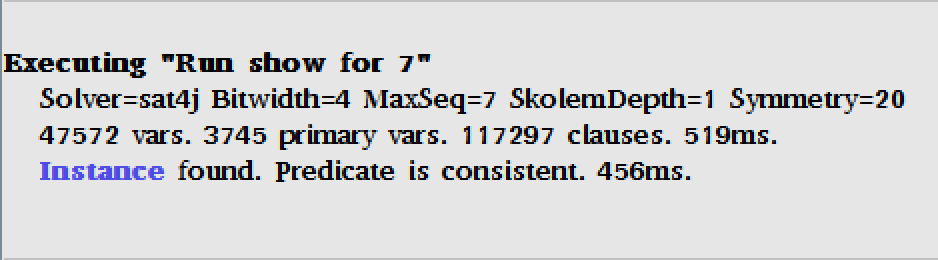
\includegraphics[scale=0.8]{alloy_run.png}
\label{fig:alloy_run}
\caption{Execution Details.}
\end{figure}

\begin{figure}[H]
\centering
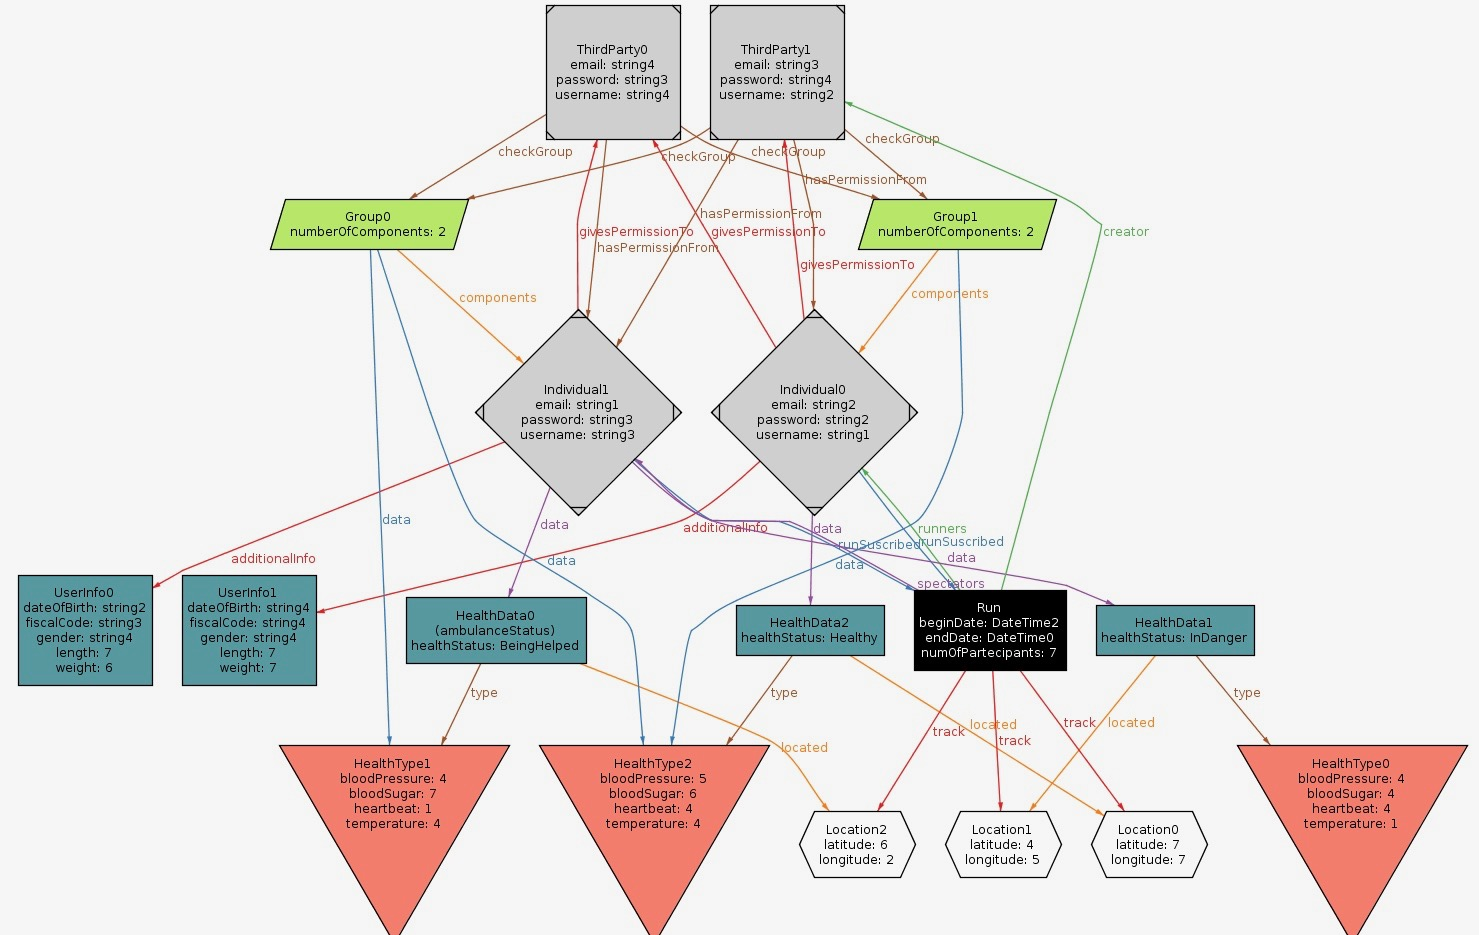
\includegraphics[scale=0.38, angle=-90, origin=c]{world1.jpeg}
\label{fig:world1}
\caption{Generated World 1.}
\end{figure}

\begin{figure}[H]
\centering
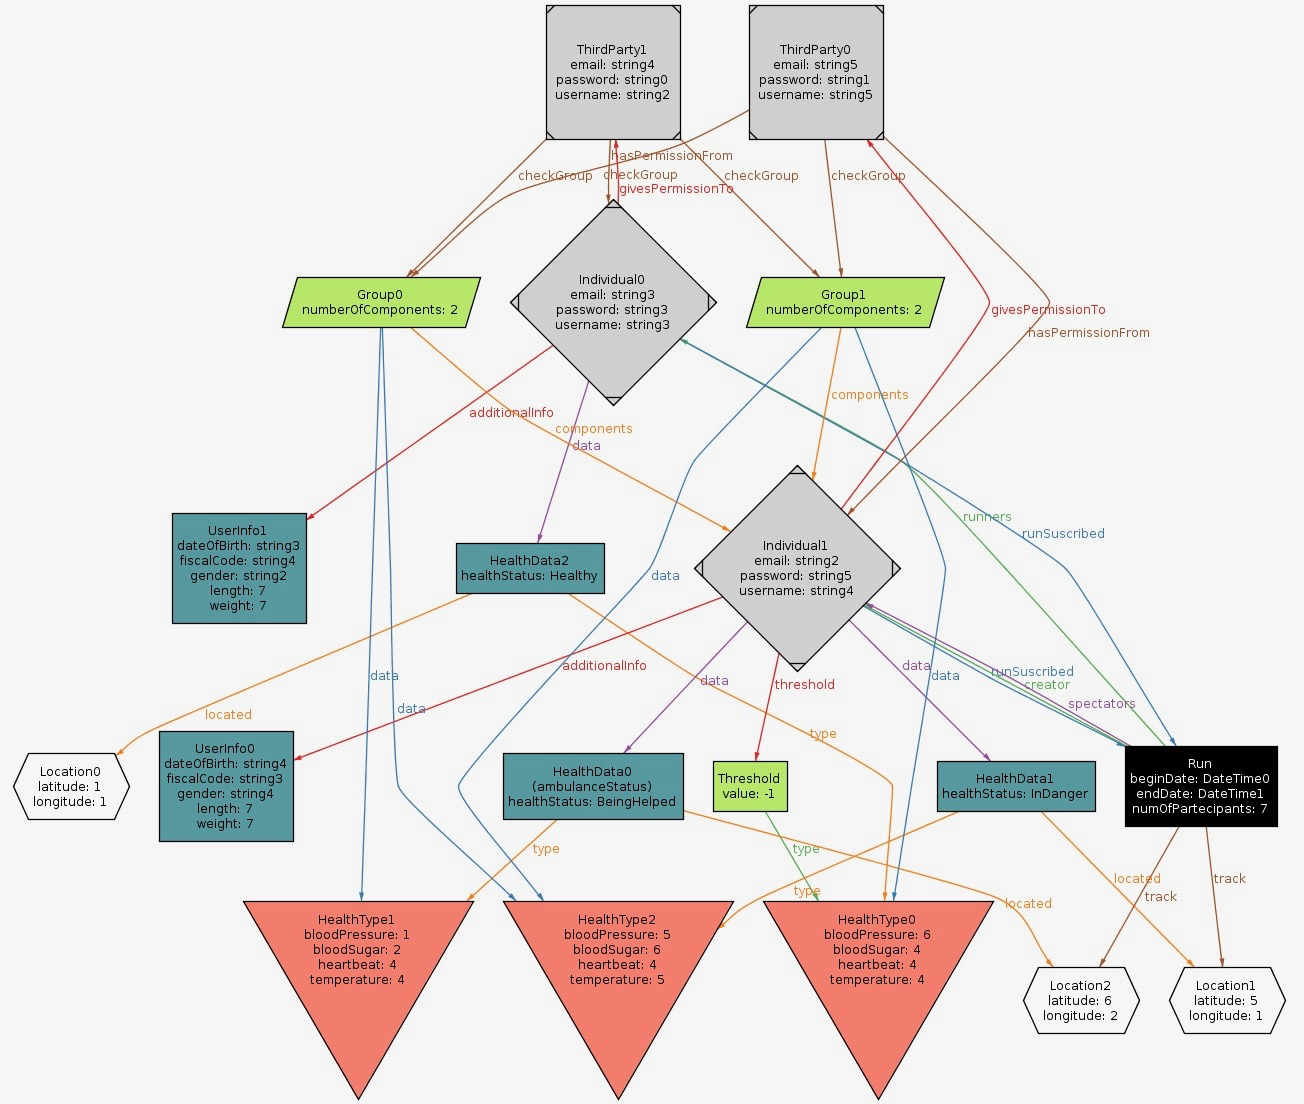
\includegraphics[scale=0.41, angle=-90, origin=c]{world2.jpeg}
\label{fig:world2}
\caption{Generated World 2.}
\end{figure}

\newpage
\section{Effort Spent}
\subsection{Michiel Janssen}

\begin{center}
\begin{tabular}{ |p{0.25\textwidth}|p{0.4\textwidth}|p{0.25\textwidth}| } 
 \hline
 \textbf{DATE} & \textbf{TASK} & \textbf{HOURS} \\ 
  \hline
  0/10/2018 & Requirements Analysis, Purpose, Scope & 2 \\ 
  \hline
  16/10/2018 & Definitions, Acronyms, Abbreviations, Scope, Document Structure & 2 \\ 
  \hline
  18/10/2018 & Product Perspective, Goals, Domain Assumptions & 3,5 \\ 
  \hline
  19/10/2018 & User Interfaces (Mockups), Hardware Interfaces & 3,5 \\ 
  \hline
  21/10/2018 & User Interfaces (Mockups), Product Functions, User Characteristics, Software Interfaces, Communication Interfaces, Domain Assumptions, Functional Requirements & 5 \\ 
  \hline
  22/10/2018 & Functional Requirements, Class Diagram, Use Case Diagrams, Use Case Description & 7 \\ 
  \hline
  24/10/2018 & Team discussion and start Alloy & 1 \\ 
  \hline
  28/10/2018 & State Diagrams, Alloy & 3 \\ 
  \hline
  03/11/2018 & Alloy & 4,5 \\ 
  \hline
  11/11/2018 & Alloy, text changes & 3,5 \\ 

  \hline
  \textbf{TOTAL} & \multicolumn{2}{c|}{35} \\ 
  \hline
\end{tabular}
\end{center}


\subsection{Erbol Kasenov}

\begin{center}
\begin{tabular}{ |p{0.25\textwidth}|p{0.4\textwidth}|p{0.25\textwidth}| } 
 \hline
 \textbf{DATE} & \textbf{TASK} & \textbf{HOURS} \\ 
  \hline
  18/10/2018 & Goals, Domain Assumptions, State Diagrams & 3\\ 
  \hline
  20/10/2018 & Hardware Limitations, User Characteristics,Product Function & 2 \\ 
  \hline
  23/10/2018 & Product Function ,State Diagrams & 2 \\ 
  \hline
  24/10/2018 & Team discussion and start Alloy & 1 \\ 
  \hline
  04/11/2018 & Common state diagram, Security,  Maintainability,  Portability & 3 \\
  \hline
  \textbf{TOTAL} & \multicolumn{2}{c|}{11} \\ 
  \hline
\end{tabular}
\end{center}

\subsection{Lorenzo Casalini}

\begin{center}
\begin{tabular}{ |p{0.25\textwidth}|p{0.4\textwidth}|p{0.25\textwidth}| } 
 \hline
 \textbf{DATE} & \textbf{TASK} & \textbf{HOURS} \\ 
  \hline
  18/10/2018 & Goals, Domain Assumptions, State Diagrams & 3,5\\ 
  \hline 
  20/10/2018 & State Diagrams, Activity Diagrams & 3 \\
  \hline
  22/10/2018 & Functional Requirement, Performance Costraints & 3.5 \\
  \hline
  23/10/18 & Use Case Descriptions, Software System Attributes & 2.5 \\
  \hline
  24/10/2018 & Team discussion and start Alloy & 2 \\ 
  \hline
  25/10/2018 & Alloy & 2.5 \\ 
  \hline
  29/10/2018 & Alloy & 2 \\ 
  \hline 
  30/10/2018 & Alloy & 2.5\\
  \hline
  5/11/2018 & Alloy & 3.5 \\ 
  \hline
  \textbf{TOTAL} & \multicolumn{2}{c|}{25} \\ 
  \hline
\end{tabular}
\end{center}


\section{Used Tools}
\begin{itemize}
    \item Papeeria (online latex)
    \item StarUML 3.0.2
    \item Adobe Photoshop
    \item Alloy Analyzer 5.0.0
\end{itemize}


\end{document}
